 \documentclass[11pt,a4paper]{article}

\usepackage[margin=1in, paperwidth=8.3in, paperheight=11.7in]{geometry}
\usepackage[ruled, vlined, linesnumbered]{algorithm2e}
\usepackage{amsfonts}
\usepackage{amsmath}
\usepackage{amssymb}
\usepackage{dsfont}
\usepackage{enumerate}
\usepackage{enumitem}
\usepackage{fancyhdr}
\usepackage{graphicx}
\usepackage{tikz}
\usepackage{changepage} 

\usepackage[utf8]{inputenc}
\usepackage{listings}
\usepackage{xcolor}

\lstset{
    frameround=fttt,
    language=Prolog,
    numbers=left,
    breaklines=true,
    mathescape=true,
    keywordstyle=\color{blue}\bfseries, 
    basicstyle=\ttfamily\color{red},
    numberstyle=\color{black}
    }

\begin{document}

\pagestyle{fancy}
\setlength\parindent{0pt}
\allowdisplaybreaks

\renewcommand{\headrulewidth}{0pt}
\setlist[enumerate,1]{label={\roman*)}}

% Cover page title
\title{Advanced Algorithms - Notes}
\author{Dom Hutchinson}
\date{\today}
\maketitle

% Header
\fancyhead[L]{Dom Hutchinson}
\fancyhead[C]{Advanced Algorithms - Notes}
\fancyhead[R]{\today}

% Counters
\newcounter{definition}[section]
\newcounter{example}[section]
\newcounter{notation}[section]
\newcounter{proposition}[section]
\newcounter{proof}[section]
\newcounter{remark}[section]
\newcounter{theorem}[section]

% commands
\newcommand{\dotprod}[0]{\boldsymbol{\cdot}}
\newcommand{\cosech}[0]{\mathrm{cosech}\ }
\newcommand{\cosec}[0]{\mathrm{cosec}\ }
\newcommand{\sech}[0]{\mathrm{sech}\ }
\newcommand{\prob}[0]{\mathbb{P}}
\newcommand{\nats}[0]{\mathbb{N}}
\newcommand{\cov}[0]{\mathrm{Cov}}
\newcommand{\var}[0]{\mathrm{Var}}
\newcommand{\expect}[0]{\mathbb{E}}
\newcommand{\reals}[0]{\mathbb{R}}
\newcommand{\integers}[0]{\mathbb{Z}}
\newcommand{\indicator}[0]{\mathds{1}}
\newcommand{\nb}[0]{\textit{N.B.} }
\newcommand{\ie}[0]{\textit{i.e.} }
\newcommand{\eg}[0]{\textit{e.g.} }
\newcommand{\X}[0]{\textbf{X}}
\newcommand{\x}[0]{\textbf{x}}
\newcommand{\iid}[0]{\overset{\text{iid}}{\sim}}
\newcommand{\proved}[0]{$\hfill\square$\\}
\newcommand{\Mod}[1]{\ \mathrm{mod}\ #1}

\newcommand{\definition}[1]{\stepcounter{definition} \textbf{Definition \arabic{section}.\arabic{definition}\ - }\textit{#1}\\}
\newcommand{\definitionn}[1]{\stepcounter{definition} \textbf{Definition \arabic{section}.\arabic{definition}\ - }\textit{#1}}
\newcommand{\proof}[1]{\stepcounter{proof} \textbf{Proof \arabic{section}.\arabic{proof}\ - }\textit{#1}\\}
\newcommand{\prooff}[1]{\stepcounter{proof} \textbf{Proof \arabic{section}.\arabic{proof}\ - }\textit{#1}}
\newcommand{\example}[1]{\stepcounter{example} \textbf{Example \arabic{section}.\arabic{example}\ - }\textit{#1}\\}
\newcommand{\examplee}[1]{\stepcounter{example} \textbf{Example \arabic{section}.\arabic{example}\ - }\textit{#1}}
\newcommand{\notation}[1]{\stepcounter{notation} \textbf{Notation \arabic{section}.\arabic{notation}\ - }\textit{#1}\\}
\newcommand{\notationn}[1]{\stepcounter{notation} \textbf{Notation \arabic{section}.\arabic{notation}\ - }\textit{#1}}
\newcommand{\proposition}[1]{\stepcounter{proposition} \textbf{Proposition \arabic{section}.\arabic{proposition}\ - }\textit{#1}\\}
\newcommand{\propositionn}[1]{\stepcounter{proposition} \textbf{Proposition \arabic{section}.\arabic{proposition}\ - }\textit{#1}}
\newcommand{\remark}[1]{\stepcounter{remark} \textbf{Remark \arabic{section}.\arabic{remark}\ - }\textit{#1}\\}
\newcommand{\remarkk}[1]{\stepcounter{remark} \textbf{Remark \arabic{section}.\arabic{remark}\ - }\textit{#1}}
\newcommand{\theorem}[1]{\stepcounter{theorem} \textbf{Theorem \arabic{section}.\arabic{theorem}\ - }\textit{#1}\\}
\newcommand{\theoremm}[1]{\stepcounter{theorem} \textbf{Theorem \arabic{section}.\arabic{theorem}\ - }\textit{#1}}

\tableofcontents

% Start of content
\newpage

\section{Hashing}

\definition{Dictionary}
A \textit{Dictionary} is an abstract data structure which stores $(\textit{key},\textit{value})$ pairs, with \textit{key} being unique.\\
A \textit{Dynamic Dictionary} can perform the following operations
\begin{center}
\begin{tabular}{l|l}
\textbf{Operation}&\textbf{Description}\\\hline
\lstinline!add(k,v)!&Add the pair \lstinline!(k,v)!.\\
\lstinline!lookup(k)!&Return \lstinline!v! if \lstinline!(k,v)! is in dictionary, \lstinline!NULL! otherwise.\\
\lstinline!delete(k)!&Remove pair \lstinline!(k,v)!, assuming \lstinline!(k,v)! is in dictionary.
\end{tabular}
\end{center}
A \textit{Static Dictionary} can only perform lookups, after it has been built.
\begin{center}
\begin{tabular}{l|l}
\textbf{Operation}&\textbf{Description}\\\hline
\lstinline!lookup(k)!&Return \lstinline!v! if \lstinline!(k,v)! is in dictionary, \lstinline!NULL! otherwise.
\end{tabular}
\end{center}

\proposition{Implementing a Dictionary}
Many data structures can be used to implement a \textit{Dictionary}.\\
These include, but not limited to:
\begin{enumerate}
	\item Linked lists.
	\item Binary Search, (2,3,4) \& Red-Black Trees.
	\item Skip lists
	\item van Emde Boas Trees.
\end{enumerate}

\remark{Motivation for Hashing}
None of the implementations of a \textit{Dictionary} suggested in \textbf{Proposition 1.1} achieves a $O(1)$ run-time complexity in the worst case for \underline{all} operations. To achieve this we introduce \textit{Hashing}.\\

\definition{Hash Function}
A \textit{Hash Function} takes in object's key and returns a value which is used to index the object in a \textit{Hash Table}.\\
Let $S$ be the set of all possible keys a hash function can recieve \& $m$ be the number of indexes in its \textit{Associated Hash Table}. Then
$$h:S\to[m]$$
\nb We want to avoid cases where $h(x)=h(y)$ for $x\neq y$(\textit{collisions}) .\\

\remark{Hashing functions assign items to indices with a geometric distribution}

\remark{Avoiding Collisions in Hashing}
When indexing $n$ items to $m$ indicies using a \textit{Hash Function} we only avoid \textit{Collisions} if $m\gg n$.\\

\definition{Hash Table}
A \textit{Hash Table} is an abstract data structre which extends the \textit{Dictionary} in such a way that time complexity is reduced.\\
A \textit{Hash Table} is comprise of an array \& a \textit{Hash Function}. The \textit{Hash Function} maps an object's key to an index in the array. If multiple objects have the same \textit{Hash Value} then a \textit{Linked List} is used in that index, with new objects added to the end of the \textit{Linked List} (Called \textit{Chaining}).\\

\proposition{Time Complexity for Dictionary Operations in a Hash Table}
By building a \textit{Hash Table} with \textit{Chaining} we achieve the following time complexities for \textit{Dictionary} operations
\begin{center}
\begin{tabular}{l|l|l}
\textbf{Operation}&\textbf{Worst Case Time Complexity}&Comments\\\hline
\lstinline!add(k,v)!&$O(1)$&Add item to the end of \textit{Linked List} if necessary.\\
\lstinline!lookup(k)!&$O($length of chain containing \lstinline!k!$)$&We might have to search through the whole\\&&\textit{Linked List} containing \lstinline!k!.\\
\lstinline!delete(k)!&$O($length of chain containing \lstinline!k!$)$&Only $O(1)$ to perform the actual deletion,\\
&&but need to find \lstinline!k! first.
\end{tabular}
\end{center}

\theorem{True Randomness}
Consider $n$ fixed inputs for a \textit{Hash Table} with $m$ indices. (\ie any sequence of $n$ \lstinline!add!/\lstinline!lookup!/\lstinline!delete! operations).\\
Pick a \textit{Hash Function}, $h$, at random from a set of all \textit{Hash Functions}, $H:=\{h:S\to[m])$. Then
$$\expect(\text{Run-Time per Operation})=O\left(1+\frac{n}{m}\right)$$
\nb The expected run-time per operation is $O(1)$ if $m\gg n$.\\

\proof{Theorem 1.1}
Let $x\ \&\ y\in S$ be two distincy keys \& $T$ be a \textit{Hash Table} with $m$ indexes.\\
Define $I_{x,y}\begin{cases}1&h(x)=h(y)\\0&\text{otherwise}\end{cases}$.\\
We have $\prob(h(x)=h(y))=\frac{1}{m}$.\\
Therefore
\[\begin{array}{rcl}
\expect(I_{x,y})&=&\prob(I_{x,y}=1)\\
&=&\prob(h(x)=h(y))\\
&=&\frac{1}{m}
\end{array}\]
Let $N_x$ be the number of keys stored in $H$ that are hashed to $h(x)$.\\
Note that $N_x=\displaystyle\sum_{k\in T}I_{x,k}$.\\
Now we have that
$$\expect(N_x)=\expect\left(\displaystyle\sum_{k\in T}I_{x,k}\right)=\sum_{k\in H}\expect(I_{x,k})=n\frac{1}{m}=\frac{n}{m}$$
\proved

\remark{Why not hash to unique values}
Suppose we want to define a \textit{Hash Function} which maps each key in $S$ to a unique position in the \textit{Hash Table}, $T$. This requires $m$ unique positions, which in turn require $\log_2 m$ bits for each key. This is an unreasonably large amount of space.\\

\proposition{Specifying the Hash Function}
Consider a set of \textit{Hash Functions}, $H:=\{h_1,h_2,\dots\}$.\\
When we initialise a \textit{Hash Table} we choose a hash function $h\in H$ at random and then proceed only to use $h$ when dealing with this specific \textit{Hash Table}.\\

\remark{Randomness in Hashing}
All the randomness in \textit{Hashing} comes from how we choose the \textit{Hash Function} \& not from how the \textit{Hash Function} itself runs.\\

\definition{Weakly Universal Set of Hashing Functions}
Let $H:=\{h|h:S\to[m]\}$ be a set of \textit{Hashing Functions}.\\
$H$ is \textit{Weakly Universal} if for any chosen $x,y\in S$ with $x\neq y$
$$\prob(h(x)=h(y))\leq\frac{1}{m}\text{ when varying }h(\cdot)$$
when $h$ is chosen uniformly at random from $H$.\\

\theorem{Expected Run time for Weakly Universal Set}
Consider $n$ fixeds to a \textit{Hash Table}, $T$, with $m$ indexes.\\
Pick a \textit{Hash Function}, $H$, from a \textit{Weakly Universal Set} of \textit{Hash Functions}, $H$.
$$\expect(\text{Run-Time per Operation})=O(1)\text{ for }m\geq n$$
\nb Proof is same as for \textit{True Randomness}.\\

\proposition{Constructing a Weakly Universal Set of Hash Functions}
Let $S:=[s]$ be the set of possible keys \& $p$ be some prime greater than $s$\footnote{There is a theorem that $\forall\ n\ \exists\ p\in[n,2n]$ st $p$ is prime.}.\\
Choose some $a,b\in[0,p-1]$ \& define
\[\begin{array}{rcl}
h_{a,b}(x)&=&\underbrace{[\ (ax+b)\Mod p\ ]}_\text{spread values over [0,p-1]}\underbrace{\Mod m}_\text{causes collisions}\\
H_{p,m}&=&\{h_{a,b}(\cdot):a\in[1,p-1],\ b\in[0,p-1]
\end{array}\]
\nb $H_{p,m}$ is a \textit{Weakly Universal Set} of \textit{Hashing Functions}.\\
\nb Different values of $a\ \&\ b$ perform differently for different data sets.\\

\remarkk{True Randomness vs Weakly Universal Hashing}
\begin{itemize}
	\item[-] For both \textit{True Randomness} \& \textit{Weakly Universal Hashing} we have that when $m\geq n$ the expected \lstinline!lookup! time in the \textit{Hash Table} is $O(1)$.
	\item[-] Constructing a \textit{Weakly Universal Set} of \textit{Hash Functions} is generally easier.
\end{itemize}

\theorem{Longest Chain - True Randomness}
If \textit{Hashing Function} $h$ is selected uniformly at random from all \textit{Hashing Functions} to $m$ indicies.\\
Then, over $m$ inputs we have
$$\prob(\exists\text{ a chain length}\geq3\log_2 m)\leq\frac1m$$

\proof{Theorem 1.3}
This problem is equivalent to showing that if we randomly throw $m$ balls into $m$ bins the probabiltiy of having a bin with at least $3\log_2 m$ balls is at most $\frac1m$.\\
Let $X_1$ be the number of valls in the first bin.\\
Choose any $k$ of the $M$ balls, the probabiltiy that all of these $K$ balls go into the first bin is $\frac1{m^k}$.\\
By the \textit{Union Bound Theorem} we have
$$\prob(X_1\geq k)\leq{m\choose k}\frac{1}{m^k}\leq1{k!}$$
Applying the \textit{Union Bound Theorem} again we have
$$\prob(\text{at least 1 bin recieves at least }k\text{ balls})\leq m\prob(X_1\geq k)\leq\frac{m}{k!}$$
Observe that
\[\begin{array}{rcl}
k!&>&2^{k-1}\\
\text{Let }k&=&3\log_2 m\\
\implies k!&>&2^{(3\log_2m-1)}\\
&\geq&2^{2\log_2 m}\\
&\geq&(2^{\log_2 m})^2\\
&=&m^2
\end{array}\]
Thus, setting $k=3\log_2 m$ means
$$\frac{m}{k!}\leq\frac1m\text{ for }m\geq2$$
\proved

\theorem{Longest Chain - Weakly Universal Hashing}
Let \textit{Hashing Function} $h$ be picked uniformly at random from a \textit{Weakly Universal Set} of \textit{Hashing Functions}.\\
Then, over $m$ inputs
$$\prob(\exists\text{ a chain length}\geq1+\sqrt{2m})\leq\frac12$$
\nb This is a poor bound.\\

\proof{Theorem 1.4}
Let $x,y\in S$ be two keys and define $I_{x,y}\begin{cases}1&h(x)=h(y)\\0&\text{otherwise}\end{cases}$.\\
Let $C$ be a random variable for the total number of collision (\ie $C=\sum_{x,y\in H, \x<y}I_{x,y}$).\\
Using \textit{Linearity of Expectation} and that $\expect(I_{x,y})=\frac1m$ when $h$ is \textit{Weakly Universal}
$$\expect(C)=\expect\left(\sum_{x,y\in H,\ x<y}I_{x,y}\right)=\sum_{x,y\in H,\ x<y}\expect(I_{x,y})={m\choose2}\frac1m\leq\frac{m}{2}$$
By \textit{Markov's Inequality}
$$\prob(C\geq m)\leq\frac{\expect(C)}m\leq\frac12$$
Let $L$ be a random variable for the length of the longest chain in $H$.\\
Then, $C\leq{L\choose2}$.
Now
$$\prob\left(\frac{(L-1)^2}{2}\geq m\right)\leq\prob\left({L\choose2}\geq m\right)\leq\prob(C\geq m)\leq\frac12$$
By rearranging, we have that
$$\prob(L\geq1+\sqrt{2m})\leq\frac12$$

\subsection{Perfect Hashing}

\remark{Motivation}
The \textit{Hashing Schemes} discussed in the previous part perform well in the best \& average cases but not necessarily in the worst cases (as they can have really long longest chains).\\

\definition{Static Perfect Hashing}
A \textit{Perfect Static Hashing Scheme} is a scheme that produces a \textit{Hash Table} where  \lstinline!lookup! has time complexity $\in O(1)$, even in the worst case. However this \textit{Hash Table} is static so we cannot perform \lstinline!insert! or \lstinline!delete! after the table has been produced.\\
\nb \textit{FKS Hashing Scheme} is a \textit{Perfect Static Hashing Scheme}.\\

\definition{FKS Hashing Scheme}
Below is an algorithm for the \textit{FKS Hashing Scheme}\\
\begin{algorithm}[H]
\SetKwInOut{Require}{require}
\caption{FKS Hashing Scheme}
\Require{$n \{\text{\# insertions}\}, T \{\text{Table with $n$ entries}\}$}
Insert all $n$ into $T$ using $h$\\
\While{Collisions in $T\geq n$}{
	Rebuild $T$ using a new $h$.
}
Let $n_i=|T[i]|$.\\
\For{$i\in[1,n]$}{
	Insert items of $T[i]$ into new table $T_i$ of size $n_i^2$ using $h_i$.\\
	\While{Collisions in $T_i\geq 1$}{
		Rebuild $T_i$ using a new $h_i$.
	}
}
\Return{T}
\end{algorithm}
\nb $\prob(\text{Collisions in }T_i\geq1)\leq\frac12$ and \nb $\prob(\text{Collisions in }T\geq n)\leq\frac12$ so we expect to have to build each table twice.\\

\remark{If $n$ items are mapped to the same index this counts as ${n\choose2}$ collision.}

\proposition{FKS Hashing Scheme - \lstinline!lookup!}
Below is an algorithm for \lstinline!lookup(x)! in the \textit{Hash Tables} produced by the \textit{FKS Hashing Scheme}
\begin{algorithm}[H]
\caption{FKS - \lstinline!lookup(x)!}
\SetKwInOut{Require}{require}
\Require{$T\ \{\text{main table}\}, \{T_1,\dots,T_m\}\ \{\text{sub-tables}\},x\ \{\text{key}\}$}
Compute $i=h(x)$.\\
Compute $j=h_i(x)$.\\
\Return{$T_i[j]$}
\end{algorithm}
\nb This runs in $O(1)$ time.\\

\proof{FKS Hashing Scheme - Space Requirements}
In the \textit{FKS Hashing Scheme} the main table $T$ requires space $O(n)$ and each sub-table $T_i$ requires space $O(n_i^2)$, where $n_i=|T[i]|$.\\
Storing each task function, $h_i$ requires space $O(1)$.\\
Thus the total space used is1
$$O(n)+\sum_iO(n_i^2)=O(n)+O\left(\sum_in_i^2\right)$$
We know there are ${n_i\choose 2}$ collisions in $T[i]$ so there are $\sum_i{n_i\choose 2}$ collisions in $T$.\\
We know there are at most $n$ collisions in $T$ so
$$\sum_i\frac{n_i^2}{4}\leq\sum_i{n_i\choose2}<n\implies\sum_in_i^2<4n$$
Thus
$$O(n)+O\left(\sum_in_i^2\right)=O(n)$$

\proof{FKS Hashing Scheme - Expected Construction Time}
The expected construction time for the main table, $T$, is $O(n)$.\\
The expected construction time for reach sub-table, $T_i$, is $O(n_i^2)$ where $n_i:=|T[i]|$.\\
Thus
\[\begin{array}{rcl}
expect(\text{construction time})&=&{\displaystyle\expect\left(\text{construction time of }T+\sum_i\text{construction time of }T_i\right)}\\
&=&\expect\text{construction time of }T)+{\displaystyle\expect\left(\sum_i\text{construction time of }T_i\right)}\\
&=&O(n)+{\displaystyle\sum_iO(n_i^2)}\\
&=&O(n)+{\displaystyle O\left(\sum_in_i^2\right)}\text{ see Proof 1.4}\\
&=&O(n)
\end{array}\]

\propositionn{FKS Hashing Scheme - Properties}
\begin{itemize}
	\item[-] Has no collisions.
	\item[-] \lstinline!lookup! takes $O(1)$ time in worst-case.
	\item[-] Uses $O(n)$ space.
	\item[-] Can be build in $O(n)$ expected time.
\end{itemize}

\subsection{Cuckoo Hashing}

%TODO something about bucketing
\remark{}
If our consruction has the property that $\forall\ x,y\in S$ with $x\neq y$ the probabiltiy that $x$ and $y$ are in the same bucket is $O\left(\frac1m\right)$, then for any $n$ operations the expected run-time is $O(1)$ per operation.\\

\definition{Cuckoo Hashing}
In \textit{Cuckoo Hasing} we use two hash functions, $h_1\ \&\ h_2$, to produce a single hash table.\\
When we \lstinline!add! a value $x$ to the hash table we place it in position $h_1(x)$. If there is already a value, $y$, already in this position then we move that value, $y$, to its alternative positione. We keep moving values until each value is in its position. If it is not possible (\ie we have found a cycle) then we change $h_1\ \&\ h_2$ for new hash functions and rehash all the values.\\
This is formally descibed in the algorithm below\\
\begin{algorithm}[H]
\SetKwInOut{Require}{require}
\caption{Cuckoo Hashing - Insert}
\Require{$\{x_1,\dots,x_n\}$ $\{\text{stream of keys}\}$, $T\ \{\text{Table with $m$ entries}\}$}
\textbf{choose} $h_1,h_2$
\For{$i\in[1,n]$}{
	$pos=h_1(x)$.\\
	$checked=[]$.\\
	\While{$T[pos]$ not empty}{
		\lIf{$x\in checked$}{\textbf{rehash}}
		$checked$ append $x$.
		$y=T[pos]$.\\
		$T[pos]=x$.\\
		$pos=$alternative position for $y$.\\
		$x=y$.
	}
	$T[pos]=x$.
}
\Return{T}
\end{algorithm}
\nb \textit{Rehash} involves chooseing two new hash functions $h_1\ \&\ h_2$ are reinserting all keys, $\{x_1,\dots,x_n\}$ into the table.\\

\propositionn{Cuckoo Hashing Scheme - Properties}
\begin{enumerate}
	\item An \lstinline!add! takes \textit{amortised exepcted} time $O(1)$.
	\item Every \lstinline!lookup! and every \lstinline!delete! has time complexity $O(1)$ in the worst-case.
	\item The space requirement is $O(n)$ where $n$ is the number of keys stored.
\end{enumerate}

\remark{Assumptions in Cuckoo Hashing}
In \textit{Cuckoo Hashing} we make the following assumptions
\begin{enumerate}
	\item $h_1$ and $h_2$ are indepenent.\\
	\ie $h_1(x)$ says nothing about $h_2(x)$, and visa-versa.
	\item $h_1$ and $h_2$ are truly random.\\
	\ie They map to each entry in the hash table with uniform probability.
	\item Computing the value of $h_1(x)$ and $h_2(x)$ takes $O(1)$ time in the worst-case.
\end{enumerate}

\definition{Cuckoo Graph}
A \textit{Cuckoo Graph} is an interprettation of a \textit{Hash Table} using \textit{Graph Theory}.\\
Each vertex of the graph is an entry in the hash table and for each $x_i$ we add an undirected-edge between $h_1(x_i)$ and $h_2(x_i)$.\\
If any cycles occur in a \textit{Cucko Graph} then we know construction will fail for that pair of hash functions as no stable scenario can occur.\\
The length of the longest path tells us the time for the longest insert.\\

\theorem{Probability of Long Paths in Cuckoo Graphs}
Let $m$ be the size of a hash table \& $n$ the number of entries we wish to insert
Fr any pair of positions $i$ and $j$, and any constant $c>1$, if $m\geq2cn$ then the probability that there exists a shortest path in the cuckoo graph from $i$ to $j$ with length $l\geq1$ is at most $\frac1{c^lm}$.\\

\proof{Theorem 1.5}
TODO\\

\proof{Probability of a path between two positions in a Cuckoo Graph}
If a path exists from $i$ to $j$, ther emust be a shortest path from $i$ to $j$.\\
Therefore we can use \textbf{Theorem 1.5} and the \textit{Union Bound} over all possible paths to show the probability of a path from $i$ to $j$ existing is at most
$$\sum_{l=1}^\infty\frac1{c^lm}=\frac1m\sum_{l=1}^\infty\frac1{c^l}=\frac1m\frac1{c-1}=O\left(\frac1m\right)$$

\definition{Buckets}
We say that two keys $x\ \&\ y$ are in the same \textit{bucket} iff there exists a path from $h_1(x)$ to $h_1(y)$ in a \textit{Cuckoo Graph}.\\
Note that this implies there is a path from $h_1(x),h_2(y)$; $h_2(x),h_1(y)$ and $h_2(x),h_2(y)$ as there are edges $(h_1(x),h_2(x))$ \& $(h_1(y),h_2(y))$.\\

\remark{The time for an operation on $x$ is bounded by the number of items in its bucket.}

\proposition{Probabiltiy of being in the same Bucket}
For $x,y\in S$ with $x\neq y$ the probability that they are in the same bucket is at most
$$\sum_{l=1}^\infty\frac1{c^lm}=\frac1m\sum_{l=1}^\infty\frac1{c^l}=\frac1m\frac1{c-1}=O\left(\frac1m\right)$$
If the size of a hash table is $m\geq2cn$ then the expeceted time per operation is $O(1)$.\\
Further, \lstinline!lookup!s take $O(1)$ time in the worst case.\\

\proposition{Probability of Rehashing}
The probabiltiy that a rehashing occurs in \textit{Cuckoo Hashing} is equal to the probability of the \textit{Cuckoo Graph} having a cycle.\\
A cycle is a path from $x$ to $x$, via some intermidiary vertices.\\
Thus the probability that $x$ is involved in a cycle is
$$\sum_{l=1}^\infty\frac1{c^lm}=\frac1{m(c-1)}$$
by \textbf{Proof 1.7}.\\
Thus the probabiltiy that there is at least one cycle in the whole hash table is
$$m\frac1{m(c-1)}=\frac1{c-1}$$

\proposition{Construction Time - Cuckoo Hashing}
Consider the result in \textbf{Proposition 1.9} when $c=3$.\\
The probability of a rehashing occuring is $\frac12$.\\
Thus we expected only one rehash to be necessary. The the expected time for a rehash is $O(n)$ then the expeceted construction time for the table is $O(n)$.\\
Therefore the \textit{amortised expeced} time for rehashes over $n$ insertions is $O(1)$ per insertion.\\
\nb Checking for a cycle in a graph takes $O(n)$ time.

\section{Bloom Filters}

\definition{Bloom Filter}
A \textit{Bloom Filter} is a data structure which is designed to be a space efficient way of storing a set $S$.\\
\textit{Bloom Filters} support only the following operations
\begin{center}
\begin{tabular}{l|l}
\textbf{Operation}&\textbf{Description}\\\hline
\lstinline!insert(k)!&Insert the key \lstinline!(k)!.\\
\lstinline!member(k)!&Returns \lstinline!true! if \lstinline!(k)!$\in S$, no otherwise.
\end{tabular}
\end{center}
Note that there is no way to remove objects from a \textit{Bloom Filter} \& you cannot ask which keys are in the \textit{Bloom Filter}, only whether a particular key is.\\
\nb \textit{Bloom Filters} are meant to be used in cases where the size of the sample space is much larger than the number of keys being stored.\\

\remark{Motivation}
\textit{Bloom Filters} can be used to build a blacklist of unsafe URLS. Whenever a new unsafe URL, \lstinline!k!, is discovered we add it to the filter, \lstinline!insert(k)!.\\
Whenever we want to visit to a new URL, \lstinline!k!, we can query whether it is in the bloom filter, \lstinline!member(k)!, and if we are returned \textit{yes} then it is blocked.\\

\remark{Randomness in Bloom Filter}
A \textit{Bloom Filter} is randomised in such a way that \lstinline!member(k)! will sometimes return \textit{yes} when in fact \lstinline!k!$\not\in S$. However it will never return \textit{no} if \lstinline!k!$\in S$.\\
\nb The amount of space used by a \textit{Bloom Filter} depends on the failure rate we allow it.\\

\proposition{Usefullness of Bloom Filter}
For a \textit{Bloom Filter} \lstinline!insert(k)! \& \lstinline!member(k)! both run in $O(1)$ and it requries $O(n)$ bits of space to store up to $n$ keys.\\

\proposition{Building a Bloom Filter - Array}
A na\"ive approach to building a \textit{Bloom Filter} is to use an array.\\
Suppose we have sample space $1,2,\dots,|U|$ for key values.\\
We can store a set by mainting a bit string $B$ where $B[k]=1$ if $k\in S$ and $B[k]=0$ otherwise.\\
\eg \begin{tabular}{|c|c|c|c|c|c|}
\hline
1&2&3&4&5&6\\\hline
0&1&0&0&0&1\\\hline
\end{tabular} here $|U|=6$ and $S=\{2,6\}$.\\
The \textit{Bloom Filter} operations take $O(1)$ time but the array is $|U|$ long.\\

\proposition{Building a Bloom Filter - Hash Table}
Let $h:U\to[1,m]$ be a hash function.\\
We can implement a \textit{Bloom Filter} using a \textit{Hash Table} is we define that performing \lstinline!insert(k)! sets $B[h(k)]=1$ and \lstinline!member(k)! returns $\mathtt{true}$ if $B[h(k)]==1$, and $\mathtt{false}$ otherwise.\\
Using a hash function means the bit string $B$ being maintained is much shorter than if we used the \textit{Array} approach in \textbf{Proposition 2.2}, however we now have to deal with collisions \& thus false-positive results from \lstinline!member(k)!.\\
\nb false-positives occur \lstinline!member(k)! if $\exists k'\in S$ st $h(k')=h(k)$.\\

\remark{Reducing Collisions - Bloom Filter as Hash Table}
To ensure a low probability of collisions each operation, we pick the hash function $h$ at random (Note that we don't change $h$ after it is set).\\

\proposition{Probability of False Positive - Bloom Filter as Hash Table}
Suppose we have inserted $n$ keys into the \textit{Bloom Filter} and now we perform \lstinline!member(k)! for $k\not\in S$.\\
The bit string $B$ contains at most $n$ 1s among its $m$ positions.\\
By definition the hash function assigns values uniformly $\prob(h(i)=j)=\frac1m$ for $k\in[1,m]$.\\
Thus the probability of a false-positive is $\prob(B[h(k)]=1)\leq\frac{n}m$.\\
If we choose $m$ to be $100n$ then $\prob(B[h(k)]=1)\leq.01$.\\

\proposition{Bloom Filter Complexities}
Both \lstinline!insert(k)! and \lstinline!member(k)! run in $O(1)$ and the structure uses $m$ bits.\\
If we want a .01 false positive rate then $100n$ bits are required.\\

\proposition{Building a Bloom Filter - Proper}
Again we are maintaining a bit string $B$ of length $m<|U|$.\\
Let $h_1,\dots,h_r$ be $r$ hash functions which map $U\to[1,m]$ uniformly at random.
\begin{itemize}
	\item[-] \lstinline!insert(k)! sets $B[h_i(k)]=1$ for \underline{all} $i\in[1,r]$.
	\item[-] \lstinline!member(k)! returns $\mathtt{true}$ iff $B[h_i(k)]=1\ \forall\ i\in[1,r]$.
\end{itemize}

\proposition{Probability of False Positive for \textbf{Proposition 2.6}}
Assume that we have inserted $n$ keys into the \textit{Bloom Filter} and that we are performing \lstinline!member(k)! for $k\not\in S$.\\
This checks whether $B[h_i(k)]=1\ \forall\ i\in[1,r]$.\\
This is question whether $r$ randomly chosen bits of $B$ all equal 1 due to hash functions being uniformly random.\\
As there are $n$ keys in the \textit{Bloom Filter} at most $nr$ bits of $B$ are set to 1.\\
So $\frac{nr}{m}$ is the proportion of bits set to $1$ in $B$.\\
So the probability that a ranomly chosen bit is $1$ is $\leq\dfrac{nr}{m}$.\\
Thus the probability that $r$ randomly chosen bits are all equal to 1 is $\leq\left(\dfrac{nr}{m}\right)^r$.\\

\proposition{Minimising False Positive Rate}
By differentiating $\leq\left(\dfrac{nr}{m}\right)^r$ we find it is minimised for $r=\frac{m}{ne}$.\\
If we substitute this back in we get a false positive rate of at most $\left(\frac1e\right)^{\frac{m}{ne}}\approx(0.69)^\frac{m}{n}$.\\
So for a failure rate of $1\%$ we set $m\approx12.52 n$.\\
This is much better than $m=100n$ required for \textbf{Proposition 2.4}.\\

\remark{Limitations of Hashing}
Using \textit{Hashing} for dynamic dictionaries has a few draw backs
\begin{enumerate}
	\item Randomness.
	\item Amortisation, \ie expected complexities are averaged over $n$.
	\item Inflexible, hard to add new operations.
\end{enumerate}

\section{van Emde Boas Trees}

\proposition{New operations for Dynamic Dictionary}
Below are some operations which are often used as an extension to the \textit{Dynamic Dictionary} in \textbf{Definition 1.1}.
\begin{center}
\begin{tabular}{l|l}
\textbf{Operation}&\textbf{Description}\\\hline
\lstinline!predecessor(k)!&Return the pair \lstinline!(x,v)! in the dictionary\\
&with the largest key,  \lstinline!x!, such that \lstinline!x!$\leq$\lstinline!k!.\\
\lstinline!successor(k)!&Return the pair \lstinline!(x,v)! in the dictionary\\
&with the smallest key,  \lstinline!x!, such that \lstinline!x!$\geq$\lstinline!k!.\\
\end{tabular}
\end{center}
\nb \textit{Hashing}-based dynamic dictionaries are not suited to these operations.\\

\proposition{Implementing New Operations}
We could use self-balancing binary trees such as \textit{2-3-4 Trees}, \textit{Red-Black Trees} or \textit{AVL Trees}.\\
These can perform all five operations of our extended dynamic dictionary each in $O(\log n)$ worst case time and $O(n)$ space.\\

\definition{Van Emde Boas Trees}
\textit{Van Emde Boas Trees} can support the five operations of our \textit{Extended Dynamic Dictionary}.\\
\textit{Van Emde Boas Trees} can perform each operation in $O(\log\log u)$ time and use $O(u)$ space where $u$ is the size of the universe.\\
\nb Also known as \textit{vEB Trees}.\\

\proposition{vEB Trees - Array}
Suppose we wishing to store the set $S\subset U$ keys with $u=|U|$.\\
Let $A$ be a binary array of size $u$ where $A[i]=1$ iff $i\in S$.\\
We can use the following schema for each operation of the \textit{Extended Dynamic Dictionary}
\begin{enumerate}
	\item \lstinline!add(x)! - Set $A[x]=1$.
	\item \lstinline!delete(x)! - Set $A[x]=0$.
	\item \lstinline!lookup(x)! - Return $\mathtt{true}$ if  $A[x]=1$, $\mathtt{false}$ otherwise.
	\item \lstinline!predecessor(x)! - Increase $i$ until \lstinline!lookup(x-i)! returns $\mathtt{true}$. Return $x-i$.
	\item \lstinline!successor(x)! - Increase $i$ until \lstinline!lookup(x+i)! returns $\mathtt{true}$. Return $x+i$.
\end{enumerate}
Here \lstinline!add!, \lstinline!delete! \& \lstinline!lookup! take $O(1)$ time, but \lstinline!predecessor! \& \lstinline!successor! take $O(u)$ time. (Not great).\\

\proposition{vEB Trees - Blocks}
Let $S\subset U$ where $U$ is a universe of size $u$.\\
Let $B_1,\dots,B_{\sqrt{u}}$ be bit vectors of length $\sqrt{u}$ which define sequential blocks of $U$.\\
Each of these vectors stores the values $\{0,\dots,\sqrt{u}-1\}$. $B_i[j]\equiv1$ iff $x:=j+\sqrt{u}\cdot i$ is in $S$.\\
Let $C$ be a bit vector of length $\sqrt{u}$ which summaries the blocks $B_1,\dots,B_{\sqrt{u}}$.\\
We have that $C[i]\equiv1$ iff block $B_i$ is non-empty.\\
With this set up be can fulfil the oeprations as follows
\begin{itemize}
	\item[\lstinline!add(x)!]
	\begin{enumerate}
		\item Define $i:=\lfloor x/\sqrt{u}\rfloor$ \& $j:=x-i\cdot\sqrt{u}$.
		\item Set $B_i[j]=1$ \& $C[i]=1$.
	\end{enumerate}
	\item[\lstinline!delete(x)!]
	\begin{enumerate}
		\item Define $i:=\lfloor x/\sqrt{u}\rfloor$ \& $j:=x-i\cdot\sqrt{u}$.
		\item Set $B_i[j]=0$.
		\item Check if $B_i$ is empty. If so set $C[i]=0$.
	\end{enumerate}
	\item[\lstinline!successor(x)!]
	\begin{enumerate}
		\item Define $i:=\lfloor x/\sqrt{u}\rfloor$ \& $j:=x-i\cdot\sqrt{u}$.
		\item Look for successor to $x$ in $B_i$, starting at $B_i[j]$.
		\item If no successor exists
		\begin{enumerate}
			\item Find succesor to $j$ in $C$, starting at $C[j+1]$.
			\item Return smallest element in that block.
		\end{enumerate}
	\end{enumerate}
\end{itemize}
\nb In practive the blocks are implemented as a single bit-vector.\\

\remark{\lstinline!successor(x)! for Blocks Implementation}
In the block implementation of \textit{vEB Trees} we have $T(u)=3T(\sqrt{u})+O(1)$ as we make 3 recursive calls to \lstinline!successor()!.\\
This gives time complexity $T(u)\in O(\sqrt{u})$.\\
We can improve this by reducing the number of recursive calls made.\\
To do this we restructure the data structure. (See \textbf{Proposition 3.5}).\\

\proposition{vEB Trees - Proper}
Consider the same set up as in \textbf{Proposition 3.4}.\\
Here the data structure is augment such that for each block $B_i$ we store the $\mathtt{max}$ and $\mathtt{min}$ indexes used in it.\\
By doing this we can perform \lstinline!successor(x)! as follows
\begin{enumerate}
	\item Define $i:=\lfloor x/\sqrt{u}\rfloor$ \& $j:=x-i\cdot\sqrt{u}$.
	\item If $j>\mathtt{max}_i$: \# No successor in block
	\begin{enumerate}
		\item $k=$\lstinline!$\text{successor}_C(i)$! \# Find block with next value
		\item return $B_k[\mathtt{min}_k]$
	\end{enumerate}
	\item Else: \# Successor is in block
	\begin{enumerate}
		\item return \lstinline!$\text{successor}_{B_i}(j)$!
	\end{enumerate}
\end{enumerate}
We are now only ever making a single recurisve call, giving us $T(u)=T(\sqrt{u})+O(1)$.\\
Thus $T(u)\in O(\log\log u)$.\\
\nb Each block \& summary can be defined recursively.\\

\example{vEB Trees - Proper}
Consider a universe of size $u=16$.\\
The following is an example of the datat structure that would be used
$$C=\begin{pmatrix}1\\0\\0\\1\end{pmatrix}\quad B=\begin{pmatrix}1&0&0&0\\0&0&0&0\\0&0&0&0\\0&1&0&1\end{pmatrix}\quad\mathtt{min}=\begin{pmatrix}0\\-\\-\\1\end{pmatrix}\quad\mathtt{max}=\begin{pmatrix}0\\-\\-\\3\end{pmatrix}$$
\nb Each row relates to a single block.\\

\remark{Time Complexity of \lstinline!add! for vEB Trees}
\lstinline!add! contain a single recursive call.\\
We have that $T(u)=T(\sqrt{u})+O(1)$.\\
By the Master's Theorem we have that $T(u)=O(\log\log u)$.\\
\nb This is the same for all operations.\\


\remark{Space Complexity of vEB Trees}
Let $Z(u)$ be the space use by a \textit{vEB Tree} over a universe of size $u$.\\
We have that
$$Z(u)=(\sqrt{u}+1)Z(\sqrt{u})+O(1)\implies Z(u)=O(u)$$

\section{Orthogonal Range Searching}

\definition{$nD$ Range Searching Data Structure}
An \textit{$n$-Dimensional Range Searching Data Structure} stores $m$ distinct $n$-dimensional data points and supports a single operation
\begin{center}
\begin{tabular}{l|l}
\textbf{Operation}&\textbf{Description}\\\hline
\lstinline!lookup($l_1,u_1,\dots,l_1,u_1$)!&Return all stored points $(z_1,\dots,z_n)$ where\\
&$l_1\leq z_1\leq u_1$ and $\dots$ and $l_n\leq z_n\leq u_n$.
\end{tabular}
\end{center}

\proposition{$1D$ Range Searching Data Structure}
Consider an array of stored values $[x_1,\dots,x_n]$.\\
Make a balanced binary tree by recursively taking the midpoint of the array as a new node and then partitioning the values around.\\
\lstinline!lookup($l_1,u_1$)! can be performed as follows
\begin{enumerate}
	\item Find the successor of $l_1$. Takes $O(\log n)$ time.
	\item Find the predecessor of $u_1$. Takes $O(\log n)$ time.
	\item Find the path between the successor and predecessor.
	\item For each node on path:
	\begin{enumerate}
		\item Consider its left \& right subtree in turn (if they exist).
		\item If root of subtree is in $[l_1,u_1]$ then return all values in subtree.
	\end{enumerate}
\end{enumerate}
This implementation of \lstinline!lookup($l_1,u_1$)! takes $O(\log n+k)$ time, where $k$ is the number of points to be returned, and $O(n)$ space and $O(n\log n)$ prep-time (to construct the tree).\\
\nb Runtime depends on the size of the output.\\

\proposition{$2D$ Range Searching Data Structure - Na\"ive}
Below is a na\"ive approach for performing \lstinline!lookup(lx,ux,ly,uy)!
\begin{enumerate}
	\item Find all the points with $l_x\leq x\leq u_x$ using \textbf{Proposition 4.1}.
	\item Find all the points with $l_y\leq y\leq u_y$.
	\item Find the points in both lists.
\end{enumerate}
This approach has run time $O(\log n+k_x)+O(\log n+k_y)+O(k_x+k_y)=O(n+k_x+k_y)$ where $k_x$ is the number of points found in step $i)$ and $k_y$ is the number of points found in step $ii)$.\\

\proposition{$2D$ Range Searching Data Structure - Proper}
For preprocessing build a balanced binary tree using the $x$ value of each point.\\
Here is a better implementation of \lstinline!lookup($1_x,u_x,l_y,u_y$)!.
\begin{enumerate}
	\item Find the successor to $l_x$.
	\item Find the predeccessor to $u_x$.
	\item Find the path between these two points.\\
	Each subtree on this path has the property that either \underline{all} points in the tree have $x$ values in the range $[l_x,u_x]$, or \underline{none} of them do.
	\item For each subtree where \underline{all} points have $x$ values in the range $[l_x,u_x]$.
	\begin{enumerate}
		\item Build a \textit{1D Range Searching Structure} using the $y$-coordinates of each point in the tree.
		\item Perform \lstinline!lookup($l_y,u_y$)! on this subtree.
	\end{enumerate}
\end{enumerate}

\remark{Time Complexity \textbf{Proposition 4.3}}
Steps $i)-iii)$ take $O(\log n)$ time and the length of the path between the successor \& predecessor is of length $O(\log n)$.\\
In step $iv)$ we do $O(\log n)$ 1-D lookups. Each of these takes $O(\log n+k')$ time.\\
Thus the overall run-time is $O(log^2n+k)$ as each lookup is disjoint.\\
\nb Preprocessing takes $O(n\log n)$ time.\\

\remark{Space Complexity \textbf{Proposition 4.3}}
The initial 1D structure used $O(n)$ space.\\
At each node we stored an array containing the points in its subtree.\\
The tree has depth $O(\log n)$.\\
Thus the total space used is $O(n\log n)$.

\section{Pattern Matching}

\definition{Exact Pattern Matching Problem}
Let $T,P$ be strings of length $n,m$ respectively.\\
The \textit{Exact Pattern Matching Problem} is to find all occurences of $P$ in $T$.\\
$P$ matches at location $i$ iff $\forall\ j\in[0,m)\ P[j]=T[i+j]$.

\proposition{Na\"ive Algorithm}
A \textit{Na\"ive Algorithm} for solving the \textit{Exact Pattern Matching Problem} is to align $P$ with the start of $T$; compare every character; return if a match has occured; slide on by one character; repeat until end of $T$ is reached.\\
\nb This takes $O(nm)$ time.\\

\proposition{Proper Algorithms}
Proper Algorithms can solve the \textit{Exact Pattern Matching Problem} (\eg KMP) in $O(n)$ time.\\
Note that this mean run times depends on the size of the text being analysed, not on the pattern which is being searched for.\\

\remark{Preprocessing}
Since the text, $T$, is constant across all queries, it is acceptable to do a significant amount of preprocessing in order to speed up query times.

\subsection{Suffix Trees}

\definition{Suffix}
A \textit{Suffix} is any substring of a string which includes the last character.\\

\definition{Atomic Suffix Tree}
An \textit{Atomic Suffix Tree} is a tree where each edge is a labled by a character \& each leaf is labelled with the index at which a given suffix starts.\\
Each root-to-leaf path is a suffix in the tree.\\

\example{Atomic Suffix Tree}
Below is an \textit{Atomic Suffix Tree} for `bananas'.
\begin{center}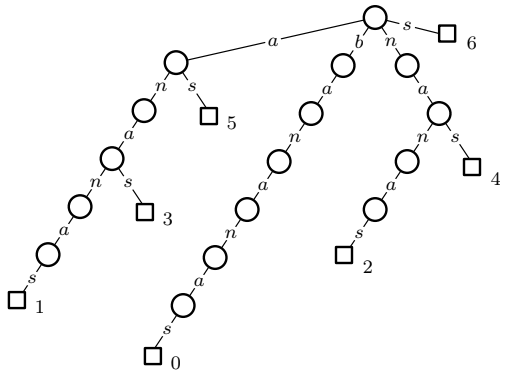
\includegraphics[scale=.5]{img/atomic_suffix_tree.png}\end{center}

\proposition{Searching a Atomic Suffix Tree}
We can use an \textit{Atomic Suffix Tree} to solve the \textit{Exact Pattern Matching Problem}.\\
Given an pattern $P$, starting at the root, step down the path dictated by $P$.\\
If $P$ requires a step which cannot be fulfilled then that pattern does not exist anywhere in $T$.\\
If the path of $P$ does terminate successfully on a node: return all the leaf values in this nodes subtree.\\

\remark{Runtime}
This approach has runtime complexity of $O(m)$.\\
It should be noted that the number of choices we have to check at each node does affect the runtime, however for constant size alphabets this is not of great concern.\\

\remark{Limitations of Atomic Suffix Tree}
\textit{Suffix Trees} can have upto $\left(\frac{n}2+1\right)^2$ internal nodes, meaning its space requirements are $O(n^2)$ are quickly become unmanageable.\\
They can contain long paths.\\

\definition{Compacted Suffix Tree}
A \textit{Compacted Suffix Tree} has the same structure as an \textit{Atomic Suffix Tree}, the only difference being that any non-branching nodes (\ie nodes with only one child) are merged into the node below and edges are now labelled with Substrings.\\
This means that every node has at least $2$ children and we have $O(n)$ edges.\\
\nb In practice we do not store the substring for each edge but rather the endpoints in $T$ in order to save space.\\

\example{Compact Suffix Tree}
Below is an \textit{Compact Suffix Tree} for `bananas'.
\begin{center}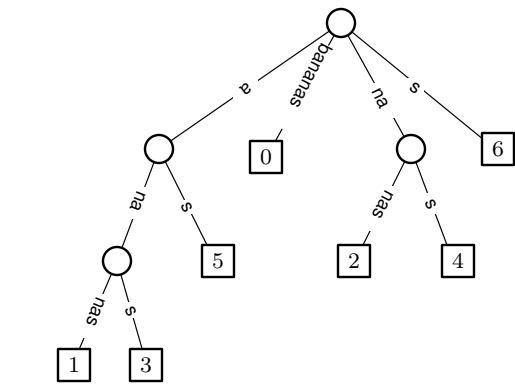
\includegraphics[scale=.5]{img/compact_suffix_tree.png}\end{center}

\proposition{A Compact Suffix Tree does \textbf{not} always exist}
A complete \textit{Compact Suffix Tree} does not always exist.\\
Suppose $T=$`$bb$' then the tree would contain a single edge and we would not successfully detect the pattern $P=$`$b$'.\\
This can be fixed by adding a character which does not appear in $T$ onto the end (\eg $T=$`$bb\$$').

\proposition{Searching a Compact Suffix Tree}
Same process as for an \textit{Aromic Suffix Tree} except we are comparing multiple characters at a time.\\
Run time is $O(m+\#\text{occurences})$.\\

\propositionn{Constructing a Compact Suffix Tree - Na\"ive}
\begin{enumerate}
	\item Insert the suffixes one at a time, longest to shortest:
	\begin{enumerate}
		\item Search for the new suffix in the partial suffix tree.\\
		(Same technique as pattern matching).
		\item Add a new edge and leaf for the new suffix.\\
		This may require the breaking of an edge into two.
	\end{enumerate}
\end{enumerate}
This has run-time complexity $O(n^2)$.\\
\nb This can be done in $O(n)$ time but is not covered on this course.\\

\proposition{Multiples Texts}
If we want to be able to search multiple texts we a character to the end of each text: this characters must be different \& not appear in any of the texts.\\
We then append these texts and treat them as a single text.

\subsection{Suffix Arrays}

\definition{Lexicographical Sorting}
\textit{Lexicographical Sorting} is a way of ordering words in alphabetical order.\\
Let $T_1$ and $T_2$ be two texts which we are sorting.
\begin{itemize}
	\item Compare $T_1$ \& $T_2$ character-by-character.
	\item Let $i$ be the index of the first character to differ between $T_1$ \& $T_2$.
	\item If $T_1[i]<T_2[i]$ alphabetically (or any order defined ordering) then $T_1$ is placed first, and visa-versa.
	\item If no characters differ but $T_1$ is shorter than $T_2$, then $T_1$ is placed first and visa-versa.
\end{itemize}
\nb This is how words are sorted in the dictionary.\\

\definition{Suffix Array}
Let $T$ be a text with $|T|=n$.\\
Lexicographic sort all $n$ suffices of $T$.\\
We define a \textit{Suffix Array}, $A$, st
$$A[i]=n-\text{length of suffix with was }i^\text{th}\text{ in lexicographic order}$$

\example{Suffix Array}
Consider the word \textit{`bananas'}.
\begin{center}
\begin{tabular}{|r|l|}
\hline
$n-l$&\textbf{suffix}\\\hline
0&bananas\\
1&ananas\\
2&nanas\\
3&anas\\
4&nas\\
5&as\\
6&s\\
\hline
\end{tabular}\quad
\begin{tabular}{|r|l|}
\hline
$n-l$&\textbf{suffix}\\\hline
\hline
1&ananas\\
3&anas\\
5&as\\
0&bananas\\
2&nanas\\
4&nas\\
6&s\\
\hline
\end{tabular}
\end{center}
Thus, in this case, $A=[1,3,5,0,2,4,6]$.\\

\remark{Suffix arrays are much smaller than Suffix Trees}

\proposition{Suffix Array from Suffix Tree}
If we already have a \textit{Suffix Tree} constructed then we can construct a \textit{Suffix Array} by performing a depth first search on the tree and setting $A[i]$ to be the $i^\text{th}$ element to be returned by this search.\\
\nb Depth first search can be done in $O(n)$ time.\\

\proposition{Searching a Suffix Array}
Let $T$ be a text we wish to search and $P$ be the pattern we are looking for.\\
Let $A$ be the \textit{Suffix Array} of $T$.\\
Due $A$ being ordered (lexicographically) we can perform a binary search on it to find occurences of $P$.\\
At each node we check we compare characters: if $P$ is matched completly then we can return the index of the occurence.\\
\nb Binary search can be used to find the first \& last occurence of $P$ and thus all occurences.\\

\remark{Runtime Seaching a Suffix Tree}
Comparing two strings takes $O(m)$ (where $|P|=m$) and the binary search checks $O(\log n)$ nodes (where $|T|=n$).\\
Thus overall runtime complexity for finding one occurence is $O(m\log n)$ and to find \underline{all} occurences is $O(m\log n+\#\text{occurences})$.\\
\nb This can be improved to $O(m+\log n+\#\text{occurences})$ using \textit{LCP Queries}, which are discussed later.\\

\proposition{DC3 Method}
Let $T$ be a text with $n=|T|$.\\
The \textit{DC3 Method} is an algoirthm for building \textit{Suffix Arrays} in $O(n)$.\\
First we build a \textit{Suffix Array} for two-thirds of the text \& then for the final third.
\begin{enumerate}
	\item Construct \textit{Suffix Array} for two-thirds ($S_{1,2}$):
	\begin{enumerate}
		\item Define $B_1:=\{i\in[0,n):i\ \%\ 3\equiv1\}$ \& $B_2:=\{i\in[0,n):i\ \%\ 3\equiv2\}$.
		\item Define $R_1:=T[1,\dots,n]$ \& $R_1:=T[2,\dots,n]$.
		\item Pad the ends of $R_1$ \& $R_2$ with a filler character (`\$') until their length is a multiple of 3.
		\item Split $R_1$ \& $R_2$ into blocks of length 3.
		\item Define $R:=R_1*R_2$ (Concatenation) \& split it into blocks of length 3.
		\item Label the blocks of $R$ in lexicographical order. (Takes $O(n)$ time with Radix Sort).
		\item Define $R'$ st $R'[i]=$ position of block $i$ in lexicographical order. (\nb $|R'|=\frac{2n}{3}$)
		\item Compute the \textit{Suffix Array} of $R'$.\\
		\nb This is a recursive step \& we are now sorting number suffices rather than letter suffices.
	\end{enumerate}
	\item Relabel the \textit{Suffix Array} of $R'$ in terms of first index (in $T$) of each block. (Call this $S_{1,2}$)\\
	\nb This gives the \textit{Suffix Array} of $B_1\cup B_2$.
	\item Construct \textit{Suffix Array} for other third ($S_0$):
	\begin{enumerate}
		\item Define $B_0:=\{i\in[0,n):i\ \%\ 3\equiv0\}$.
		\item Write each suffix which is indexed by $B_0$ as the first character \& the position of the suffix started by the next character in $S_{1,2}$.
		$$\underbrace{T[B_0[i]]}_\text{char}+\mathtt{index\_of}(B_0[i]+1\mathtt{\ in\ }S_{1,2})\equiv T[B_0[i]]+\mathtt{index\_of}(B_1[i]\mathtt{\ in\ }S_{1,2})$$
		\item Sort these pairs lexicographically ($O(n)$ time in Radix Sort).\\
		\item Relabel this array in terms of the index of the first character (in $T$). (Call this $S_0$).\\
		\nb This is the \textit{Suffix Array} of $B_0$.
	\end{enumerate}
	\item Merge the \textit{Suffix Array}s to form $S$:
	\begin{enumerate}
		\item Set $i=0$ and $j=0$.
		\item Compare $S_0[i]$ with $S_{1,2}[j]$:
		\begin{itemize}
			\item[\textbf{If}] $(T[S_0[i]]<T[S_{1,21}[j]])$: Insert $S_0[i]$ into $S$, increment $i$.
			\item[\textbf{Elif}] $(T[S_0[i]]>T[S_{1,2}[j]])$: Insert $S_{1,2}[j]$ into $S$, increment $j$.
			\item[\textbf{Else}]: (\ie $T[S_0[i]]\equiv T[S_{1,2}[j]]$)
			\begin{itemize}
				\item[\textbf{If}] $S_0[i]+1\in S_{1,2}$ \underline{and} $S_{1,2}[j]+1\in S_{1,2}$:
				\item Add the element associated to whichever of these indices occurs first in $S_{1,2}$. Increment $i$ or $j$ as appropriate.
				\item[\textbf{Else}] \text{Add the element associated to whichever of $S_0[i]+2$ \& $S_{1,2}[j]+2$ occurs first in $S_{1,2}$.} Increment $i$ or $j$ as appropriate.\\
				\nb These indicies are guaranteed to be in $S_{1,2}$ due to the use of $mod\ 3$.
				
			\end{itemize}
		\end{itemize}
		\item Repeat until all characters have been positioned.\\
		\nb This is very similar to \textit{Merge-Sort Merging}.
	\end{enumerate}
\end{enumerate}

\proposition{DC3 Method - Run Time}
In the \textit{DC3 Method} we have a recursive step at i) (h) which acts of two-thirds of the data.\\
The construction of $S_0$ takes $O(n)$ time as it uses \textit{Radix Sorting}.\\
The merging of $S_0$ \& $S_{1,2}$ takes $O(n)$ time.\\
Thus the \textit{DC3 Method} has run-time equation $T(n)=T\left(\frac{2}{3}n\right)+O(n)\implies T(n)\in O(n)$.

\section{Range Minimum Queries}

\definition{Range Minimum Query Problem}
Let $A$ be an array of length $n$ and $i,j\in[0,n)$ with $i<j$.\\
A \textit{Range Minimum Query} of indices $i,j$, $RMQ(i,j)$, outputs the index of the samllest value in the subarray $A[i,j]\equiv\big\{A[i],A[i+1],\dots,A[j-1],A[j]\big\}$.\\

\remark{Aim}
This can be na\"ively be done in $O(n^2)$ space \& $O(1)$ query time if we precompute a matrix of all solutions.\\
We want to do this in $O(n)$ space, $O(n)$ preprocessing time \& $O(1)$ query time.\\

\proposition{Solution 1 - Block Decomposition}
Let $A$ be an array of $n$ elements.\\
The \textit{Block Decomposition Solution} suggests preprocessing a \textit{Minimum Binary-Heap} where each node gives the value \& index of the smallest value of the leaves in its subtree.
\begin{enumerate}
	\item Define $A_1:=A$.
	\item For $i\in[1,\log_2n]$:
	\begin{enumerate}
		\item Let $k:=2^i$.
		\item Define $A_k$ st $\forall\ i\in[0,\frac{n}k],\ A_k[i]=(x,v)$ where $v:=\min(A[ik,(i+1)k])$ and $x$ is the position of $v$ in $A$.
	\end{enumerate}
\end{enumerate}
This takes $O(n)$ space since $\sum_{i=0}^\infty\frac{n}{2^i}=2n$.\\
Each layer requires $\frac{n}k$ comparisons, thus preprocessing takes $O(n)$ time.\\

\proposition{Solution 1 - Querying}
Consider performing $RMQ(i,j)$ using the heap produced by \textbf{Proposition 6.1}
\begin{enumerate}
	\item Find the largest block which lies completely within $[i,j]$.\\
	\ie The node with the largest subtree which lies completely in the $[i,j]$.
	\item Keep finding the largest block which does not overlap with any previous blocks.\\
	\item Return the minimum of root of each of these blocks.
\end{enumerate}
We will never choose 2 consequitive blocks of the same height as there will be a large block with covers them.\\
There will be no gaps in a layer (for the same reason), thus we choose at most $2$ blocks of each height.\\
Thus we pick at query at most $2\log_2n$ blocks in total.\\
Query time is $O(\log_2n)$.\\

\remark{We want faster queries}

\proposition{Solution 2 - Precompute solutions for intervals of length power of two}
Let $A$ be an array of $n$ elements.\\
Pre-compute the solutions for every interval of length $2^i$ for some $i$.
Let $A_k$ denote the array which stores the solutions to $RMQ(i,i+(k-1))\ \forall\ i$, where $k$ is a power of 2.\\
\nb $A_1:=A$.\\
$|A_k|=n-(k-1)\in O(n)$ and we have $\log_2n$ arrays so total space is $O(n\log_2n)$.\\
We can build $A_2$ from $A$ in $O(n)$ time \& $A_{2k}$ from $A_k$ in $O(n)$ so pre-processing takes $O(n\log_2n)$.\\

\proposition{Solution 2 - Querying}
Consider performing $RMQ(i,j)$ using the arrays produced by \textbf{Proposition 6.3}.
\begin{enumerate}
	\item Define $l:=j-i+1$ (The interval length).
	\item If $l$ is a power of $2$: Return $A_{l}[i]$. (\ie Just lookup the answer).\\
	\nb Takes $O(1)$ time.
	\item Otherwise:
	\begin{enumerate}
		\item Find power of two, $k$, st $k\leq l<2k$.
		\item Perform $RMQ(i,i+k-1)$ and $RMQ(j-k+1,j)$.\\
		\nb Each query takes $O(1)$ time.
		\item Return minimum of these two queries.\\
		\nb Takes $O(1)$ time.
	\end{enumerate}
\end{enumerate}
Each query can be done in $O(1)$ time.\\

\remark{Solution 2 has quicker queries but requires more space \& pre-processing time}

\proposition{Solution 3 - Low-Resolution Range Minimum Queries}
Let $A$ be an array of $n$ elements.\\
Here we replace $A$ with a \textit{lower-resolution} array $H$ and store many smaller arrays which give the detail.
\begin{enumerate}
	\item Define $\tilde{n}:=\dfrac{n}{\log_2n}$.
	\item Define $H[i]=\min(A[i\log_2n,(i+1)\log_2n-1])$ for $i\in[0,\tilde{n})$.
	\item Define sub-arrays $L_i:=A[i\log_2n,(i+1)\log_2n-1]$ for $i\in[0,\tilde{n})$.\\
	\nb In practice we just store the start \& end indices of $L_i$ and then query $A$.
\end{enumerate}
We can use \textbf{Proposition 6.3} to construct $H$.\\
This requires $O(\tilde{n}\log_2\tilde{n})=O(n)$ space \& pre-processing time, and we can perform queries in $O(1)$ time.\\
Using \textbf{Proposition 6.3} to construct each of the $L_i$ requires $O((\log_2n)\log_2\log_2n)$ space \& pre-processing time, and each can be queried in $O(1)$ time.\\
Thus, total space is $O(n)+O(\tilde{n}(\log_2n)\log_2\log_2n)=O(n\log_2\log_2n)$ \& total pre-processing time is $O(n\log_2\log_2n)$.\\

\proposition{Solution 3 - Querying}
Consider performing $RMQ(i,j)$ using the arrays produced by \textbf{Proposition 6.5}.
\begin{enumerate}
	\item Define $i':=\left\lceil\frac{i}{\log_2n}\right\rceil$ \& $j':=\left\lfloor\frac{j}{\log_2n}\right\rfloor$.
	\item Query $RMQ_H(i',j')$.
	\item If $i'\neq\frac{i}{\log_2n}$: (\ie the previous query does not cover the start of the interval)
	\begin{itemize}
		\item Query $RMQ_{L_{i'-1}}(i'-i,\log_2n)$.
	\end{itemize}
	\item If $j'\neq\frac{j}{\log_2n}$: (\ie the previous query does not cover the end of the interval)
	\begin{itemize}
		\item Query $RMQ_{L_{j'+1}}(0,j-j')$.
	\end{itemize}
	\item Return the minimum of these (at most 3) queries.
\end{enumerate}
This requires at most 3 queries, each of $O(1)$ time, so can be done in $O(1)$ time.

\subsection{$\pm1$ Range Minimum Queries}

\definition{$\pm1$ Range Minimum Query}
Let $A$ be an array of length $n$ with the property that $\forall\ k\in[0,n-1),\ A[k+1]=A[k]\pm1$.\\
Perform a \textit{Range Minimum Query} of this array.\\

\definition{Equivalent $\pm1$ Arrays}
Let $A_1$ \& $A_2$ be $\pm1$ arrays of length $n$.\\
\text{We note that the values of each index are irrelevant, \underline{only} the change in value between elements matters.}\\
Thus, $A_1$ \& $A_2$ are said to be \textit{Equivalent} if they have the same pattern of value changes.\\
\ie $A_1$ is equivalent to $A_2$ iff $\forall\ i,j\ RMQ_{A_1}(i,j)=RMQ_{A_2}(i,j)$.\\

\proposition{Number of Equivalent $\pm1$ Arrays}
Consider $\pm1$ arrays of length $n$.\\
We can denote the value change pattern of a $\pm1$ array as a binary string of length $n-1$ where the $i^\text{th}$ digit represents the value change from $A[i]$ to $A[i+1]$.\\
Let 1 denote $+1$ and 0 denote $-1$.\\
Thus there are $2^{n-1}$ unique $\pm1$ arrays of length $n$.\\

\proposition{Range Minimum Queries for $\pm1$ Arrays}
Let $A$ be a $\pm1$ array of length $n$.\\
Split $A$ into $\tilde{n}:=2\frac{n}{\log_2n}$ blocks.\\
\text{Each block is of length $n\frac{\log_2n}{2n}=\frac12\log_2n$ and is a $\pm1$ array, thus there are at most $\sqrt{n}$ different blocks}.\\
Precompute the \textit{Range Minimum Query} of each permutation \& store in a table.\\
Store type of each block in a \textit{Low-Resolution} array, $H$.\\
Querying requires a single query of $H$ \& a single query of the precomputed table of solutions.\\
Both take $O(1)$ time, so query time is $O(1)$.\\
This requires $O(n)$ space \& pre-processing time.\\
\nb This is similar to the \textit{Low-Resolution} solution given in \textbf{Proposition 6.5}.

\section{Lowest Common Ancestor}

\definition{Ancestor}
Let $T$ be a tree \& $i$ be a node in $T$.\\
\textit{Ancestors} of $i$ in $T$ are the nodes which lie on the path from $i$ to the tree-root.\\

\definition{Lowest Common Ancestor}
Let $T$ be a tree \& $i,j$ be nodes in $T$.\\
The \textit{Lowest Common Ancestor} of $i$ \& $j$ in $T$, $LCA(i,j)$, is the node furthest from the root which is also an ancestor of \underline{both} $i$ \& $j$.\\

\remark{Aim}
We want to find a solution which works in $O(n)$ space, $O(n)$ pre-processing time \& $O(1)$ query time.\\

\definition{Euler Tour}
Let $T$ be a \textit{Tree}.\\
An \textit{Eurler Tour} of $T$ is a depth-first search, where we record backtracking as well.\\
At each node take the leftmost edge which has not already been traversed, otherwise backtrack \& repeat until all edges have been traversed.\\

\proposition{Length of Euler Tour}
Let $T$ be a \textit{Tree} with $n$ nodes.\\
Since $T$ has $n$ nodes, it has $n-1$ edges.\\
In an \textit{Euler Tour} each edge is traversed twice (once in each direction) \& trivially start at the root.\\
Thus an \textit{Euler Tour} has length $2(n-1)+1=2n-1$.\\

\remark{Euler Tours start \& end on the root of the tree}

\proposition{Solution 1 - Using Range Minimum Queries}
Let $T$ be a tree with $n$ nodes \& $i,j$ be nodes in $T$.
\begin{enumerate}
	\item Label each node of the tree incrementally with $[0,n-1]$ (left-to-right, then down a layer).
	\item Follow an \textit{Euler Tour} of $T$. At each node:
	\begin{itemize}
		\item[-] Append its value on the end of $N$.
		\item[-] Append its depth on the end of $D$.
	\end{itemize}
	\item Process $D$ for \textit{Range Minimum Queries} (Using \textbf{Proposition 6.5}).
\end{enumerate}
This produces two arrays, $N$ \& $D$, each of length $2n-1$.\\
Using \textbf{Proposition 6.5} for iii) means that pre-processing time \& total-space is
$$\underbrace{O(n\log_2\log_2n)}_\text{RMQs}+\underbrace{O(n)}_\text{Euler Tour}=O(n\log_2\log_2n)$$

\proposition{Solution 1 - Quering}
Let $T$ be a \textit{Tree} with $n$ nodes and $i,j$ be nodes in $T$.\\
Let $N$ \& $D$ be the arrays produced by \textbf{Proposition 7.2}.\\
Consider making query $LCA(i,j)$ on $T$.
\begin{enumerate}
	\item Find an occurence of $i$ \& $j$ in $N$.
	\item Let $i',j'$ be the indixes of these occurences.
	\item Return $N[\underbrace{RMQ_D(i',j')}_\text{An Index}]$.\\
	\nb $RMQ(\cdot,\cdot)$ takes $O(1)$ time.
\end{enumerate}
Each of these steps takes $O(1)$ time. Overall query-time is $O(1)$.\\

\proposition{Correctness of Solution 1}
Consider \textit{Euler Tours} recursively.\\
Let $x$ be a node at depth $x$ with children $c_1,\dots,c_k$.\\
We see the \textit{Euler Tour} has recursive structure as
\begin{center}
\begin{tabular}{c|c|c|c|c|c|c|c|}
\cline{2-8}
N&x&$\vdash$Tour of $c_1\dashv$&x&$\vdash\dots\dashv$&x&$\vdash$Tour of $c_k\dashv$&x\\
\cline{2-8}
D&d&$\vdash$Tour of $c_1\dashv$&d&$\vdash\dots\dashv$&d&$\vdash$Tour of $c_k\dashv$&d\\
\cline{2-8}
\end{tabular}
\end{center}
Claim that $RMQ(i,j)=y$ iff $LCA(i,j)=y$.\\
Let $i',j'$ be any position of $i,j$ in $N$.
\begin{enumerate}
	\item Suppose $i,j$ are in the same subtree of $y$.\\
	Then $y$ is not in interval $i',j'$.\\
	Thus cannot be returned by $RMQ(i,j)$.
	\item Suppose $i,j$ are not in subtrees of $y$.\\
	Then $y$ may be in the interval $i',j'$.\\
	Since theses are not subtrees of $y$ then a node higher than $y$ will be traversed.\\
	The index of this node will be returned by $RMQ(i,j)$ over that of $y$.
	\item Suppose $i,j$ are in different subtrees of $y$.\\
	Then $y$ is in the interval $i',j'$.\\
	Since these are both subtrees of $y$, $y$ is the highest element in the trees.\\
	Thus the index of $y$ is returned by $RMQ(i,j)$.
\end{enumerate}
Thus the claim holds.\proved

\proposition{Solution 2 - $\pm1$ Range Minimum Query}
Notice that the depth array, $D$, produced by \textbf{Proposition 7.2} is a $\pm1$ array.\\
Thus we can use the results from \textbf{Section 6.1}.\\
Specifically, replace $D$ with a \textit{Low-Resolution} array as described in \textbf{Proposition 6.8}.\\
Query time remains as $O(1)$.\\
Pre-processing time \& total space is now $\underbrace{O(n)}_\text{RMQs}+\underbrace{O(n)}_\text{Euler Tour}=O(n)$.\\
This fulfils the aims in \textbf{Remark 7.1}.

\subsection{Solving Range Minimum Queries using Leach Common Ancestor}

\definition{Cartesian Tree}
Let $A$ be an array.\\
The \textit{Cartesian Tree} of is defined recursively
\begin{enumerate}
	\item Set $\min(A)$ as root.
	\item Partition $A$ around $\min(A)$ into $A_1$ \& $A_2$.
	\item Repeat for $A_1$ \& $A_2$, making the resulting trees subtrees.
\end{enumerate}
\nb This can be done in $O(n)$, but not covered.\\

\remark{$LCA(i,j)$ in the cartesian tree of $A\equiv RMQ_A(i,j)$}
This gives $O(n)$ space \& pre-processing time, and $O(1)$ query time for the \textit{Range Minimum Query} problem, using the solution to \textit{Least Common Ancestors} in \textbf{Proposition 7.5}.

\section{Approximation Algorithms}

\remark{Look at NP-Completeness}

\definition{Approximation Algorithm}
Let $A$ be an algorithm.\\
$A$ is an \textit{$\alpha$-Approximation Algorithm} for a problem, $P$, if
\begin{enumerate}
	\item $A$ runs in \textit{Polynomial-Time}.
	\item $A$ always outputs a solution with a value, $s$, within an $\alpha$ factor of the \textit{Optimal} solution.
\end{enumerate}
The measure depends on the type of problem $P$ is
\begin{itemize}
	\item If $P$ is a \textit{Maximisation Problem}, then $\dfrac{\text{Optimal}}\alpha\leq s\leq\text{Optimal}$.
	\item If $P$ is a \textit{Minimisation Problem}, then $\text{Optimal}\leq s\leq\alpha\cdot\text{Optimal}$.
\end{itemize}

\subsection{Constance Factor Approximations}

\definition{Constant Factor Approximation Algorithm}
A \textit{Constant Factor Approximation Algorithm} is an \textit{Approximation Algorithm} where the approximation value, $\alpha$, has a constant value, independent of the input.

\remark{Below are some examples of Constant Factor Approximations}

\subsubsection{Bin Packing Problem}

\definition{BinPacking Problem}
Consider an infinite number of bins of size $1$ \& a set of items with size $\in[0,1]$.\\
The \textit{BinPacking Problem} is to find the fewest number of bins required to store this set of items.\\
This is \textit{NP-Hard}.\\
The \textit{Decision} version of this problem is ``\textit{can you pack the items into $k$ bins?}".\\
The \textit{Decision} version is \textit{NP-Complete}.\\

\proposition{Solution 1 - First Fit}
We can approximate the \textit{BinPacking Problem} as
\begin{center}
\textbf{If} item $i$ fits into bin $j$: pack it; next item;\\
\textbf{else}: start new bin.
\end{center}
Let $I$ be the sum of the weights of the items, $fill(i)$ be the sum of the item sizes in bin $i$ \& $s$ be the number of bins used.\\
Using the technique above we observe that $fill(2i-1)+fill(2i)>1\ \forall\ 2i\in[1,s]$.
\[\begin{array}{rl}
\implies&\left\lfloor\frac{s}2\right\rfloor<\sum_{2i\in[1,s]}fill(2i-1)+fill(2i)\leq I<\mathtt{Opt}\\
\implies&s\leq2\cdot\mathtt{Opt}
\end{array}\]
Thus, we know that this solution uses no more that twice the optimal number of bins.\\
This is a \textit{$2$-Approximation Algorithm} of the \textit{BinPacking Problem}.\\
\nb This runs in $O(n)$ time.\\

\proposition{Solution 2 - First Fit Decreasing}
Consider sorting the items in \textit{Non-Decreasing} order, then fit each item into the left-most bin it will fit in.\\
This runs in $O(n^2)$ time and uses $s$ bins.\\
Consider bin $j=\lceil\frac{2s}3\rceil$
\begin{itemize}
	\item[Case 1] Suppose bin $j$ contains an item of size $>\frac12$.\\
	Then each bin $j'\leq j$ contains at item of size $>\frac12$.\\
	Thus at least $j=\lceil\frac{2s}3\rceil$ bins are required.\\
	Thus, $s\leq\frac32\cdot\mathtt{Opt}$.
	\item[Case 2] Suppose bin $j$ only contains times of size $\leq\frac12$.\\
	When the first item was packed into $j$ all bins $j'\in(j,s]$ were empty and all unpacked items had size $\leq\frac12$.\\
	Thus each bin $j'\in(j,s)$ contains at least 2 items and bin $s$ contains at least one item.\\
	This means at least $2(s-j)+1$ items don't fit into bins $j'\in[1,j)$.\\
	Thus $\sum$item weights$>\min\{j-1,2(s-j)+1\}\geq\lceil\frac{2s}3\rceil-1$.\\
	Since $\sum$item weights$\leq\mathtt{Opt}\implies\lceil\frac{2s}3\rceil-1\leq\mathtt{Opt}$.\\
	Thus, $s\leq\frac{3}{2}\mathtt{Opt}$.
\end{itemize}
Thus, in both cases, this solution is a \textit{$\frac32$-Approximation Algorithm}.

\subsubsection{Job Scheduling on Parallel Machines}

\proposition{Scheduling Jobs on Parallel Machines Problem}
Consider having $m$ identical machines \& $n$ jobs which vary in time taken.\\
Our goal is to minimise the time taken to process all the jobs.\\
\nb This problem is \textit{NP-Hard}.\\

\remark{Assessing Success}
Let $J$ be the set of all jobs \& $J_i$ be the set of jobs assigned to machine $i$.\\
Define $L_i:=\sum_{j\in J_i}t_j$ to be the time for machine $i$ to execute all its jobs.\\
Thus the total time to execute all jobs in $J$ is $\sup L_i$.\\
Thus we want to minimise $\sup L_i$.\\

\proposition{Solution 1 - Greedy Algorithm}
Let $J$ be the set of all jobs, with $n:=|J|$ and there be $m$ identical machines.
\begin{center}
Assign job $j$ to the machine $i$ with the current smallest load.
\end{center}
Naively this takes $O(nm)$ time to produce a schedule, but can be done in $O(n\log m)$ time using a \textit{Priority Queue}.\\
\nb This is an \textit{Online Algorithm}.\\

\proposition{Solution 1 - Approximation Value}
Let $\mathtt{Opt}$ denote the time taken by the optimal schedul \& $T$ denote the time taken by the greedy schedule produced by \textbf{Proposition 8.4}.\\
Note that $\mathtt{Opt}\geq\sup t_j$ where $t_j$ is the time taken by job $j$.\\
And, $\mathtt{Opt}\geq\frac1m\sum_jt_j$ since at least one machine will have a load $L_i\geq\frac1m\sum_jt_j$.\\
Consider the machine $i$ with the greatest load (\ie $L_i\equiv T$).\\
Let $j$ be the last job assigned to $i$.\\
We know that when $j$ was assigned to $i$, $i$ had the lighestest load (\ie $L_i-t_j\leq L_k\ \forall\ k\in[1,m]$).\\
Summing every machine we get
\[\begin{array}{rcl}
m(L_i-t_j)&\leq&\displaystyle\sum_{k=1}^mL_k\\
\implies L_i-t_j&\leq&\dfrac1m\displaystyle\sum_{k=1}^mL_k\\
&\leq&\mathtt{Opt}\text{ by second fact}
\end{array}\]
Since $t_j\leq\mathtt{Opt}$ we have
\[\begin{array}{rcl}
T&=&L_i\\
&=&L_i-t_j+t_j\\
&\leq&\mathtt{Opt}+\mathtt{Opt}\\
&=&2\ \mathtt{Opt}\\
\implies T&\leq&2\ \mathtt{Opt}
\end{array}\]
Thus \textbf{Proposition 8.4} is a $2$-Approximation.\\

\proposition{Solution 2 - Longest Processing Time}
Let $J$ be the set of all jobs, with $n:=|J|$, let $t_j$ be the time to execute job $j$ and let there be $m$ identical machines.
\begin{center}
Sort jobs in non-increasing order.\\
Put job $j$ into machine $i$ with the smallest current load.
\end{center}
This takes $O(n\log n)$ time to produce a schedule.\\

\proposition{Solution 2 - Approximation Value}
Let $J$ be the set of all jobs, with $n:=|J|$, let $t_j$ be the time to execute job $j$ and let there be $m$ identical machines.
Let $\mathtt{Opt}$ denote the time taken by the optimal schedul \& $T$ denote the time taken by the  schedule produced by \textbf{Proposition 8.6}.\\
Note that if $n\leq m$ then \textbf{Proposition 8.6} is optimal.\\
Else (if $n>m$):\\
At least one of the machines is assigned two jobs (each taking at least $t_{m+1}$ time).\\
Thus $\mathtt{Opt}\geq 2t_{m+1}$.\\
\\
Let $i$ be the machine with the greatest load. (\ie $T\equiv L_i$).\\
Let $j$ be the last job assigned to $i$. We have $L_i-t_j\leq\mathtt{Opt}$.\\
Assume $n>m$ and that $i$ has assigned at least two jobs. Then $L_i-t_j>0$.\\
We have that $t_j\leq t_{m+1}\leq\frac12\mathtt{Opt}$ (\ie the time for last job is no more than the $(m+1)^\text{th}$ job's) by previous fact.\\
Therefore
\[\begin{array}{rcl}
T&=&L-i\\
&=&L_i-t_j+t_j\\
&\leq&\mathtt{Opt}+\frac12\mathtt{Opt}\\
&=&\frac32\mathtt{Opt}\\
\implies T&\leq&\frac32\mathtt{Opt}
\end{array}\]
Thus \textbf{Proposition 8.6} is a $\frac32$-Approximation.

\subsubsection{$k$-Centres}

\proposition{$k$-Centres Problem}
Consider $n$ points in a 2D space.\\
We want to insert $k$ centres into the space st the maximum distance from any point to the closest centre is minimised.\\
\nb Distance is measured as the \textit{Euclidean Distance} $\sqrt{(x_1-x_2)^2+(y_1-y_2)^2}$.\\

\proposition{Solution 1 - Greedy Algorithm}
Let $\{x_1,\dots,x_p\}$ be some points in 2D space.\\
Here is a \textit{Greedy Algorithm} which offers a solution to \textbf{Proposition 8.8}
\begin{enumerate}
	\item Pick any point to be a centre.
	\item Pick the point which has the greatest distance to its nearest centre to be a new centre.
	\item Repeat ii) until $k$ centres have been picked.
\end{enumerate}
This takes $O(nk)$ time.\\

\proposition{Solution 1 - Approximation Factor}
Let $C$ be the set of centres produced by \textbf{Proposition 8.9} \& $C_\mathtt{Opt}$ be the optimal set of centres.\\
Let $r$ be the greatest distance of a point from its nearest centre in $C$\\
and $r_\mathtt{Opt}$ be the greatest distance of a point from its nearest centre in $C_\mathtt{Opt}$.
\begin{itemize}
	\item[Case 1]\textit{No $c_i,c_{i'}\in C$ which have the same closest centre ,$c_j$, in $C_\mathtt{Opt}$}.\\
	Then all points must be within $r_\mathtt{Opt}$ of a centre in $C_\mathtt{Opt}$.\\
	Thus all points are at most $2r_\mathtt{Opt}$ from a centre in $C$. (opposite side of circle radius $r_\mathtt{Opt}$)\\
	\item[Case 2]\textit{$\exists\ c_i,c_{i'}\in C$ which have the same closest centre ,$c_j$, in $C_\mathtt{Opt}$}.\\
	Thus $s_i$ is at most $2r_\mathtt{Opt}$ from $s_{i'}$. (opposite side of circle radius $r_\mathtt{Opt}$)\\
	Assume that $c_i$ was made a centre after $c_{i'}$, WLOG.\\
	Thus $c_i$ was the furthest from any exisiting centre in $C$ when it was added.\\
	Thus before adding $s_i$ all centres in $C$ were at most $2r_\mathtt{Opt}$ from another centre in $C$.\\
	Thus $r\leq r_\mathtt{Opt}$.
\end{itemize}
Thus \textbf{Proposition 8.9} is 1 $2$-Approximation

\subsection{Fully Polynomial Time Approximation Schemes}

\definition{Pseudo-Polynomial Time Algorithm}
An algorithm is \textit{Pseudo-Polynomial Time Algorithm} if it runs in \textit{Polynomial Time} when all the numbers are integers $\leq n^c$ for some constant $c$.\\

\definition{Polynomial Time Approximation Scheme}
A \textit{Polynomial Time Approximation Scheme}, PTAS, for a problem $P$ is a family of algorithms, $A$, st $\forall\ \varepsilon>0$ there is an algorithm $A_\varepsilon\in A$ st $A_\varepsilon$ is a $(1+\varepsilon)$-Approximation algorithm for $P$.\\
\nb A \textit{PTAS} does not have to have a time complexity which is polynomial in $1/\varepsilon$.\\

\definition{Fully Polynomial Time Approximation Scheme}
A \textit{PTAS} is called a \textit{Fully PTAS}, FPTAS, if it has a time complexity which is polynomial in $1/\varepsilon$ (as well as in $n$).

\subsubsection{Subset Sum}

\definition{Subset Sum Problem}
Let $S$ be a set of positive intergers \& $t\in\nats$ be a target value.\\
The \textit{Decision Problem} of the \textit{Subset Sum Problem} is to find if there is a subset, $S'\subseteq S$, st $\sum_{s\in S'}=t$.\\
The \textit{Optimisation Problem} of the \textit{Subset Sum Problem} is to find the size of the \underline{largest} subset, $S'\subset S$, st $\sum_{s\in S'}\leq t$. (Note the inequality).\\
\nb The \textit{Decision Problem} is \textit{NP-Hard} and the \textit{Optimisation Problem} is \textit{NP-Complete}.\\

\proposition{Solution 1 - Exact Solution for Decision Problem}
Let $S$ be a set of $m$ positive intergers \& define $S_i:=S[1,i]$ and $t\in\nats$ be a target value.\\
Let $L_i$ be the set of all total sum values of $S'\subseteq S_i$ which are \underline{no larger} than $t$.\\
Note that the largest subset of $S$ with total-sum value $\leq t$ is the largest number in $L_m$.\\
We can compute $L_i$ from $L_{i-1}$ as
$$L_i=L_{i-1}\cup\{x\in L_{i-1}:x+S[i]\leq t\}$$
There are no duplicates in $L_i$ so $|L_i|\leq t$.\\
We can now use the following algorithm
\begin{enumerate}
	\item Let $L_0=\{0\}$.
	\item For $i\in[1,m]$:
	\begin{itemize}
		\item[-] Define $L_i=L_{i-1}\cup\{x\in L_{i-1}:x+S[i]\leq t\}$.
	\end{itemize}
	\item Return $\sup L_m$.
\end{enumerate}
The overall time-complexity is $O(mt)=O(n^{c+1})$.\\
Thus this a \textit{Pseudo-Polynomial Time} algorithm.\\

\proposition{Solution 2 - PTAS}
Let $S$ be a set of $m$ positive intergers \& define $S_i:=S[1,i]$ and $t\in\nats$ be a target value.\\
Let $L_i$ be the set of all total sum values of $S'\subseteq S_i$ which are \underline{no larger} than $t$.\\
We want to construct a \textit{trimmed} version of $L_i$, $L_i'$, which is a subset of $L_i$ and whose length is polynomial in the input length (\ie $|L_i'|\leq n^c$ for some $c$).\\
We condition that $\forall\ y\in L_i\ \exists z\in L_i'$ which is almost as big as $y$.\\
We define the process $\mathtt{Trim}(\cdot,\cdot)$.
\begin{center}
$\mathtt{Trim}(L_i,\delta)$: $L_i[j]\in L_i'$ iff $L_i[j]>(1+delta)\cdot\mathtt{prev}$
\end{center}
where $\mathtt{prev}$ is the previous value we included in $L_i'$.\\
Now we have an algorithm
\begin{enumerate}
	\item Let $L_0'=\{0\}$ and $d=\frac1{2m}\varepsilon$.
	\item For $i\in[1,m]$:
	\begin{itemize}
		\item[-] Compute $U=L_{i-1}'\cup\{x\in L_{i-1}':x+S[i]\leq t\}$.
		\item[-] Define $L_i':=\mathtt{Trim}(U,\delta)$.
	\end{itemize}
	\item Return $\sup L_m'$.
\end{enumerate}
This algorithm does throw away possible subsets but will always output a \underline{valid} subset (but it may not be the largest).\\

\theorem{}
Consider the setup in \textbf{Proposition 8.12}.
\begin{center}
$\forall\ y\in L_i,\ \exists\ z\in L_i'$ st $\dfrac{y}{(1+\delta)^i}\leq z\leq y$.
\end{center}

\proof{Theorem 8.1}
\textit{Proof by induction}.\\
\underline{Base Case} - $L_0=L_0'=\{0\}$.\\
\underline{Inductive Case}: Assume \textbf{Theorem 8.1} holds for $i-1$.\\
As $y\in L_i$ we have that either $y\in L_{i-1}$ or $(y-S[i])\in L_{i-1}$:
\begin{itemize}
	\item[($y\in L_{i-1}$)] then $\exists\ x\in L_{i-1}'$ st $\dfrac{y}{(1+\delta)^{i-1}}\leq x\leq y$ by the \textit{Inductive Hypothesis}.\\
	By the definition of $\mathtt{Trim}\ \exists\ z\in L_i'$ st $z\leq x\leq z\cdot(1+\delta)$.\\
	$\implies z\leq x\leq y$ and $\dfrac{y}{(1+\delta^i)}\leq\dfrac{x}{1+\delta}\leq z$.\\
	\ie $\exists\ z\in L_i'$ st $\dfrac{y}{(1+\delta)^i}\leq z\leq y$, as required.
	\item[($y-S{[i]}\in L_{i-1}$)] Very similar to above.
\end{itemize}

\proposition{Solution 2 - Is a PTAS}
Using \textbf{Theorem 8.1} with $i:=m$ and $\delta:=\frac{1}{2m}\varepsilon$ we have that
\begin{center}
$\forall\ y\in L_m,\ \exists\ z\in L_m'$ st $\dfrac{y}{(1+\frac\varepsilon{2m})^m}\leq z\leq y$.
\end{center}
We have that $\mathtt{Opt}\in L_m$ so $\exists\ z\in L_m'$ st $\dfrac{\mathtt{Opt}}{(1+\frac\varepsilon{2m})^m}\leq z\leq\mathtt{Opt}$
For \textbf{Proposition 8.12} to be a PTAS we need to show that $(1+\frac\varepsilon{2m})^m\leq1+\varepsilon$ for $\varepsilon\in(0,1]$.
\[\begin{array}{rcl}
\left(1+\dfrac\varepsilon{2m}\right)^m&\leq&e^{\varepsilon/2}\\
&\leq&1+\dfrac\varepsilon2+\left(\dfrac\varepsilon2\right)^2\text{ since }e^x:=\sum_{i=0}^\infty\dfrac{x^i}{i!}\\
&\leq&1+\varepsilon
\end{array}\]
Thus the output of \textbf{Proposition 8.12} is some $z$ with
\[\begin{array}{rl}
&\dfrac{\mathtt{Opt}}{1+\varepsilon}\leq\dfrac{\mathtt{Opt}}{(1+\frac\varepsilon{2m})^m}\leq z\leq\mathtt{Opt}\\
\implies&\dfrac{\mathtt{Opt}}{1+\varepsilon}\leq z\leq\mathtt{Opt}
\end{array}\]
Thus \textbf{Proposition 8.12} is a valid PTAS.\\

\proposition{Solution 2 - Run-Time}
Assessing the run-time of \textbf{Proposition 8.12} amounts to assessing the size of $L_i'$.\\
By the definition of $\mathtt{Trim}$ we have that for any successive elements $z,z'\in L_i'$
$$\dfrac{z'}z\geq1+\delta=1+\frac\varepsilon{2m}$$
Further, $\forall\ z\in L_i',\ z\leq t$.
Thus, $L_i'$ contains at most $O(\log_{1+\delta}t)$ elements.\\
We have
\[\begin{array}{rcl}
|L_i'|&=&\log_{1+\delta}t\\
&=&\dfrac{ln t}{\ln(1+\frac\varepsilon{2m}}\\
&\leq&\dfrac{2m(1+\frac\varepsilon{2m})\ln t}{\varepsilon}\text{ since }\ln(1+x)>\frac{x}{x+1}\\
&=&O\left(\dfrac{m\log t}\varepsilon\right)
\end{array}\]
Thus the algorithm runs in
$$O(m|L_i'|)=O\left(m^2\frac{\log t}\varepsilon\right)=O\left(n^3\frac{\log n}\varepsilon\right)$$

\subsection{Asymptotic Polynomial Time Approximation Schemes}

\definition{Asymptotic Polynomial Time Approximation Schemes}
An \textit{Asymptotic Polynomial Time Approximation Schemes}, APTAS, for a problem $P$ is a family of algorithms $A$ where
\begin{center}
$\exists c>0$ st $\forall\ \varepsilon>0,\ A_\varepsilon\in A$ runs in polynomial-time and ouputs a solution $s$ with
\begin{itemize}
	\item[-] $\mathtt{Opt}\leq s\leq(1+\varepsilon)\mathtt{Opt}+c$ for minimisation problems.
	\item[-] $\dfrac{\mathtt{Opt}}{(1+\varepsilon)}\leq s\leq\mathtt{Opt}+c$ for maximisation problems.
\end{itemize}
\end{center}
Note that an APTAS does not have to runs polynomial in $\frac1\varepsilon$.\\

\definition{Fully Asymptotic Polynomial Time Approximation Schemes}
A \textit{Fully Asymptotic Polynomial Time Approximation Schemes}, AFPTAS, is an FPTAS which runs polynomially in $\frac{1}\varepsilon$

\subsubsection{Partition}

\definition{Partition Problem}
Let $S$ be a set of positive integers \& $t\in\nats$ be a target value.\\
The \textit{Partition Problem} is a special case of the \textit{Subset Sum Problem} where $t:=\frac{1}{2}\sum_{s\in S}s$.\\
Thus the \textit{Decision Problem} is whether there is a subset $S'\subseteq S$ st $\sum_{s'\in S'}s'=\frac{1}{2}\sum_{s\in S}s$.\\
Equivalently, can we pack $S$ into two bins of size $\frac12\sum_{s\in S}s$.\\
\nb This problem is \textit{NP-Complete}.\\

\proposition{Approximating Partition problem as BinPacking}
Here is a solution to the \textit{Partition Problem} by approximating the \textit{BinPacking Problem}.\\
We covert the \textit{Partition Problem} into a \textit{BinPacking Problem} by dividing all items \& bin sizes by $t$.\\
Now all bins have size $1$ and items $in(0,1]$.\\
If the optimal number of bins, $\mathtt{Opt}$, is 2 then the answer to the \textit{Partition Decision Problem} is $\mathtt{true}$.\\

\proposition{Solution 1 - Bin Packing}
Suppose we have $n$ items which take one of $c$ different sizes \& at most $d$ items fit in each bin, for some constants $c,d$.\\
We can describe any packing of items into a single bin by its type (the type determines num items in bin).\\
There are $i\in[0,c]$ items of any size \& $d$ different sizes. Thus
$$\text{\# types}\leq(c+1)^d$$
Ignoring rearrangements of bins we have $j\in[0,n]$ bins of each type. Thus
$$\text{\# packings}\leq(n+1)^{(c+1)^d}$$
However, not all of these are valid.\\
We can check each of the different packings to check if they are valid \& return the one with the fewest bins.\\
This takes $O(n\cdot(n+1)^{(c+1)^d})$ time \& exactly solves the \textit{BinPacking Problem}.\\

\proposition{APTAS for BinPacking}
Suppose we have $n$ items which take one of $c$ different sizes \& at most $d$ items fit in each bin, for some constants $c,d$.
\begin{enumerate}
	\item Remove all small items ($\leq\frac\varepsilon2$) so only $c=\frac2\varepsilon$ of the remaining large ($>\frac\varepsilon2$) items will fit into a single bin.
	\item Divide the items into $k=\left\lfloor n\frac{\varepsilon^2}2\right\rfloor$ a constant number of groups.\\
	The sizes of items in each group are then rounded up to match the size of the largest member (and the largest group is removed).\\
	This will leave only $d=\frac4{\varepsilon^2}$ different item sizes.
	\item Use the polynomial time algorithm to optimally pack the remaining special case.\\
	\nb This takes $O\left(n(n+1)^{(\frac4{\varepsilon^2}+1)^{2/\varepsilon}}\right)$ time.
	\item Reverse the grouping from ii) and greedily pack all the small items remvoed in i)
\end{enumerate}

\proposition{Packing Large Items}
Each large item is $>\frac\varepsilon2$ so at most $\frac2\varepsilon$ bins are required.\\

\proposition{ii) - Reducing the number of items sizes} %TODO redo this
Given a set of items, order then in non-increasing order \& split them into continuous groups of $k$ items (the last group may have less items).\\
Define $S'$ to be the set of these items but each item is rounded to the maximum size in its group \underline{and} does not include the largest group.\\
This means $S'$ contains $\frac{n}k$ distinct items.\\
By the way we define $k$, it is big enough st $\frac{n}k\leq\frac4{\varepsilon^2}$ (a constant).\\
Note that $\mathtt{Opt}_{S'}\leq \mathtt{Opt}_S\leq \mathtt{Opt}_{S'}+k$ by \textbf{Proof 8.2}.\\
\\
Setting $k:=\lfloor n(\frac{\varepsilon^2}2)\rfloor$ and $S$ to be the set of `large items'.\\
Then $k\leq\varepsilon\cdot\mathtt{Opt}_S$ since each of the $n$ items in $S$ is $\geq\frac\varepsilon2$.\\
$\implies\mathtt{Opt}_{S'}+k\leq(1+\varepsilon)\mathtt{Opt}_S$.\\
$\implies\mathtt{Opt}_S\leq\mathtt{Opt}_{S'}\leq(1+\varepsilon)\mathtt{Opt}_S$.\\

\prooff{$\mathtt{Opt}_{S'}\leq \mathtt{Opt}_S\leq \mathtt{Opt}_{S'}+k$}
\begin{itemize}
	\item[-] If $S$ can be packed into $b$ bins, then $S'$ can be packed into $b$ bins.\\
	Each item from $S$ is replaced by an item from the next group down. This item is no larger than it.\\
	Since $S'$ does not have the largest group of $S$, the elements in the smallest group of $S$ are discarded.
	So the packing is valid \& $\mathtt{Opt}_{S'}\leq\mathtt{Opt}_S$.
	\item[-] If $S'$ can be packed into $b$ bins, then $S$ can be packed into $b+k$ bins.\\
	This is because we can replace each item in $S'$ with a smaller item from $S$.\\
	This leaves the largest group in $S$ to be added, this group is of size $k$ thus at most $k$ bins are required.\\
	$\mathtt{Opt}_S\leq\mathtt{Opt}_{S'}+k$.
\end{itemize}
\nb Each of these transformations takes polynomial time.\\

\theorem{iv)}
Let $\varepsilon\in[0,1]$ and suppose we are given a packing of the items $s\in S$ with $s>\frac\varepsilon2$ (large items) into $b$ bins.\\
Then, we can pack all items in $S$ into either $b$ or $(1+\varepsilon)\mathtt{Opt}+1$ bins (in polynomial time).\\
This is done by placing small items anywhere but not starting an extra bin unless we have to.\\
$(1+\varepsilon)\mathtt{Opt}+1$ bins are required iff all the bins in the given packing (except possibly the last) is $1-\frac\varepsilon2$ full.

\newpage
\setcounter{section}{-1}
\section{Reference}

\subsection{Definitions}

\definition{Amortised Expected}
\textit{Amortised Expected} is a term for the complexity of something. It describes the total complexity to execute a sequence of instructions, divided by the number of instructions.\\
\eg If $n$ instructions take $O(n)$ time to execute completley, then the \textit{amortised expected} time is $O(1)$.\\

\definition{Decision Problem}
A \textit{Decision Problem} is a problem which is answered using either \textit{yes} or \textit{no}, only.\\

\definition{Greedy Algorithm}
A \textit{Greedy Algorithm} is an algorithm which makes locally optimal choices at each stage, with the intent of finding a global optimum.\\

\definition{Online Algorithm}
An \textit{Online Algorithm} is an algorithm which can process its input in the order it is fed into the algorithm without having the entire input available at the start.\\
This means you can keep passing more information to the algorithm.\\

\definition{Offline Algorithm}
An \textit{Offline Algorithm} requires the whole input before it beings processing. This algorithm then needs to totally rerun if you want to increase the input size.

\subsection{Probability}

\definition{Sample Space, $\Omega$}
A \textit{Sample Space} is the set of possible outcomes of a scenario. A \textit{Sample Space} is not necessarily finite.\\
\eg Rolling a dice $\Omega:=\{1,2,3,4,5,6\}$.\\

\definition{Event}
An \textit{Event} is a subset of the \textit{Sample Space}.\\
The probability of an \textit{Event}, $A$, happening is
$$\prob(A)=\sum_{x\in A}\prob(x)$$

\definition{Disjoint Events}
Let $A_1\ \&\ A_2$ be events.\\
$A_1\ \&\ A_2$ are said to be \textit{Disjoint} if $A_1\cap A_2=\emptyset$.\\

\definition{$\sigma$-Field, $\mathcal{F}$}
A \textit{Sigma Field} is the set of possible events in a given scenario.\\
A \textit{Sigma Field} must fulfil the following criteria
\begin{enumerate}
	\item $\emptyset,\Omega\in\mathcal{F}$.
	\item $\forall\ A\in\mathcal{F}\implies A^c\in\mathcal{F}$.
	\item $\forall\ \{A_1,\dots,A_n\}\subseteq\mathcal{F}\implies\bigcup\limits_{i=1}^nA_i\in\mathcal{F}$.
\end{enumerate}

\definition{Probability Measure, $\prob$}
A \textit{Probability Measure} maps a \textit{$\sigma$-Field} to $[0,1]$ which satisfies
\begin{enumerate}
	\item $\prob(\emptyset)=0$ \&\ $\prob(S)=1$; and,
	\item If $\{A_1,\dots,A_n\}\subseteq\mathcal{F}$ are pair-wise disjoint then $\prob\left(\bigcup\limits_{i=1}^nA_i\right)=\sum_{i=1}^n\prob(A_i)$. [$\sigma$-Additivity]
\end{enumerate}

\definition{Random Variable}
A \textit{Random Variable} is a function from the sample space, $S$, to the real numbers, $\reals$.\\
$$X:S\to\reals$$
The probability of a \textit{Random Variable}, $X$, taking a specific value $x$ is found by
$$\prob(X=x)=\sum_{\{a\in \Omega:X(a)=x\}}\prob(a)$$

\definition{Indicator Random Variable}
An \textit{Indicator Random Variable} is a \textit{Random Variable} which only ever takes $0$ or $1$ and is used to indicate whether a particular event has happened (1), or not (0).
$$\expect(I)=\prob(I=1)$$

\definition{Expected Value, $\expect$}
The \textit{Expected Value} of a \textit{Random Variable} is the mean value of said \textit{Random Variable}
$$\expect(X):=\sum_x x\prob(X=x)$$

\theorem{Linearity of Expected Value}
Let $X_1,\dots,X_n$ be random variables. Then
$$\expect\left(\sum_{i=1}^nX_i\right)=\sum_{i=1}^n\expect(X_i)$$

\theorem{Markov's Inequality}
Let $X$ be a non-negative random variable. Then
$$\prob(X\geq a)\leq\frac1a\expect(X)\quad\forall\ a>0$$

\theorem{Union Bound}
Let $A_1,\dots,A_n$ be \textit{Events}. Then
$$\prob\left(\bigcup\limits_{i=1}^nA_i)\right)\leq\sum_{i=1}^n\prob(A_i)$$
\nb This in an equality if the events are disjoint.\\

\proof{Union Bound}
Define \textit{Indicator RV} $I_i$ st
$$I_i:=\begin{cases}1&A_i\text{ happened}\\0&\text{otherwise}\end{cases}$$
Define \textit{Random Variable} $X:=\sum_{i=1}^nI_i$ (the number of events that happened).\\
Then
\[\begin{array}{rcl}
\prob\left(\bigcup\limits_{i=1}^nA_i)\right)&=&\prob(X>0)\\
&\leq&\expect(X)\text{ by Markov's Inequality}\\
&=&\expect\left[\displaystyle\sum_{i=1}^nI_i\right]\\
&=&\displaystyle\sum_{i=1}^n\expect[I_i]\\
&=&\displaystyle\sum_{i=1}^n\prob(I_i=1)\\
&=&\displaystyle\sum_{i=1}^n\prob(A_i1)
\end{array}\]
\proved

\subsection{NP-Completeness}

\definition{NP}
\textit{NP} is the set of \textit{Decision Problems} which we can \underline{validate} the answer of in polynomial time.\\

\definition{NP-Hard}
Let $A$ be a decision problem.\\
$A$ is \textit{NP-Hard} if $\forall\ B\in NP$, $B$ can be reduced to $A$ in polynomial time.\\
\nb This means we can solve $B$ using $A$.\\

\definition{NP-Complete}
Let $A$ be a decision problem.\\
$A$ is \textit{NP-Complete} if
\begin{itemize}
	\item[-] $A$ is in \textit{NP}.
	\item[-] $A$ is \textit{NP-Hard}.
\end{itemize}

\remark{If we can solve an NP-Complete problem we can solve all NP problems}

\definition{Weakly NP-Complete}
We say an \textit{NP-Complete} problem is \textit{Weakly NP-Complete} if there is a \textit{Pseudo-Polynomial Time} algorithm for it.\\

\definition{Strongly NP-Complete}
We say an \textit{NP-Complete} problem is \textit{Strongly NP-Complete} if it is still \textit{NP-Complete} when all numbers are integers $\leq n^c$ for some constant $c$.

\end{document}
